%% This file was auto-generated by IPython.
%% Conversion from the original notebook file:
%% REDD_House2_Analysis.ipynb
%%
\documentclass[11pt,english]{article}

%% This is the automatic preamble used by IPython.  Note that it does *not*
%% include a documentclass declaration, that is added at runtime to the overall
%% document.

\usepackage{amsmath}
\usepackage{amssymb}
\usepackage{graphicx}
\usepackage{ucs}
\usepackage[utf8x]{inputenc}

% needed for markdown enumerations to work
\usepackage{enumerate}

% Slightly bigger margins than the latex defaults
\usepackage{geometry}
\geometry{verbose,tmargin=3cm,bmargin=3cm,lmargin=2.5cm,rmargin=2.5cm}

% Define a few colors for use in code, links and cell shading
\usepackage{color}
\definecolor{orange}{cmyk}{0,0.4,0.8,0.2}
\definecolor{darkorange}{rgb}{.71,0.21,0.01}
\definecolor{darkgreen}{rgb}{.12,.54,.11}
\definecolor{myteal}{rgb}{.26, .44, .56}
\definecolor{gray}{gray}{0.45}
\definecolor{lightgray}{gray}{.95}
\definecolor{mediumgray}{gray}{.8}
\definecolor{inputbackground}{rgb}{.95, .95, .85}
\definecolor{outputbackground}{rgb}{.95, .95, .95}
\definecolor{traceback}{rgb}{1, .95, .95}

% Framed environments for code cells (inputs, outputs, errors, ...).  The
% various uses of \unskip (or not) at the end were fine-tuned by hand, so don't
% randomly change them unless you're sure of the effect it will have.
\usepackage{framed}

% remove extraneous vertical space in boxes
\setlength\fboxsep{0pt}

% codecell is the whole input+output set of blocks that a Code cell can
% generate.

% TODO: unfortunately, it seems that using a framed codecell environment breaks
% the ability of the frames inside of it to be broken across pages.  This
% causes at least the problem of having lots of empty space at the bottom of
% pages as new frames are moved to the next page, and if a single frame is too
% long to fit on a page, will completely stop latex from compiling the
% document.  So unless we figure out a solution to this, we'll have to instead
% leave the codecell env. as empty.  I'm keeping the original codecell
% definition here (a thin vertical bar) for reference, in case we find a
% solution to the page break issue.

%% \newenvironment{codecell}{%
%%     \def\FrameCommand{\color{mediumgray} \vrule width 1pt \hspace{5pt}}%
%%    \MakeFramed{\vspace{-0.5em}}}
%%  {\unskip\endMakeFramed}

% For now, make this a no-op...
\newenvironment{codecell}{}

 \newenvironment{codeinput}{%
   \def\FrameCommand{\colorbox{inputbackground}}%
   \MakeFramed{\advance\hsize-\width \FrameRestore}}
 {\unskip\endMakeFramed}

\newenvironment{codeoutput}{%
   \def\FrameCommand{\colorbox{outputbackground}}%
   \vspace{-1.4em}
   \MakeFramed{\advance\hsize-\width \FrameRestore}}
 {\unskip\medskip\endMakeFramed}

\newenvironment{traceback}{%
   \def\FrameCommand{\colorbox{traceback}}%
   \MakeFramed{\advance\hsize-\width \FrameRestore}}
 {\endMakeFramed}

% Use and configure listings package for nicely formatted code
\usepackage{listingsutf8}
\lstset{
  language=python,
  inputencoding=utf8x,
  extendedchars=\true,
  aboveskip=\smallskipamount,
  belowskip=\smallskipamount,
  xleftmargin=2mm,
  breaklines=true,
  basicstyle=\small \ttfamily,
  showstringspaces=false,
  keywordstyle=\color{blue}\bfseries,
  commentstyle=\color{myteal},
  stringstyle=\color{darkgreen},
  identifierstyle=\color{darkorange},
  columns=fullflexible,  % tighter character kerning, like verb
}

% The hyperref package gives us a pdf with properly built
% internal navigation ('pdf bookmarks' for the table of contents,
% internal cross-reference links, web links for URLs, etc.)
\usepackage{hyperref}
\hypersetup{
  breaklinks=true,  % so long urls are correctly broken across lines
  colorlinks=true,
  urlcolor=blue,
  linkcolor=darkorange,
  citecolor=darkgreen,
  }

% hardcode size of all verbatim environments to be a bit smaller
\makeatletter 
\g@addto@macro\@verbatim\small\topsep=0.5em\partopsep=0pt
\makeatother 

% Prevent overflowing lines due to urls and other hard-to-break entities.
\sloppy

\begin{document}

\subsection{INDiC: Improved Non-Intrusive load monitoring using load Division and Calibration}
\paragraph{Nipun Batra, Haimonti Dutta, Amarjeet Singh}
\subparagraph{{nipunb,haimonti,amarjeet}@iiitd.ac.in}
\subparagraph{About the dataset}
The datset contains high frequency, low frequency and raw data of 6
households in the USA. We choose House 2 for our analysis as it has
highest reported accuracy in REDD paper. Further we choose to do the
analysis of \textbf{low frequency} data. This house contains the
following appliances/circuits:

\begin{itemize}
\item
  Kitchen
\item
  Kitchen 2
\item
  Stove
\item
  Refrigerator
\item
  Dishwasher
\item
  Disposal
\item
  Washer Dryer
\item
  Microwave
\item
  Lighting
\end{itemize}

These circuits are samppled once every 3-4 seconds. Also the house
contains 2 mains which are sampled at 1 Hz.

\subparagraph{Imports}
In this section we setup the basic imports which shall be required for
performing the analysis and mention their version numbers.

\begin{codecell}
\begin{codeinput}
\begin{lstlisting}
import sys 
print "System version:",sys.version
import numpy as np
print "Numpy version:",np.version.version
import matplotlib
print "Matplotlib version:",matplotlib.__version__
import pandas as pd
print "Pandas version:",pd.__version__
from sklearn.cluster import MiniBatchKMeans, KMeans
import sklearn as sklearn
print "Scikit-learn version:",sklearn.__version__
import matplotlib.pyplot as plt
import math
import itertools
from pandas import Series,DataFrame
import json
import time
import pprint
import datetime
from copy import deepcopy

#Setting size of figures as 20*10
plt.figsize(20,10)



\end{lstlisting}
\end{codeinput}
\begin{codeoutput}
\begin{verbatim}
System version: 2.7.3 (default, Apr 10 2013, 05:13:16) 
[GCC 4.7.2]
Numpy version: 1.6.2
Matplotlib version: 1.1.1
Pandas version:
\end{verbatim}
\begin{verbatim}
0.11.1.dev-58642a6
Scikit-learn version: 0.12.1
\end{verbatim}
\end{codeoutput}
\end{codecell}
Prettifying CSS and Matplotlib plots

\begin{codecell}
\begin{codeinput}
\begin{lstlisting}
s = json.load( open("/home/nipun/bmh_matplotlibrc.json") )
matplotlib.rcParams.update(s)

matplotlib.rcParams.update({'font.size': 24})

from IPython.core.display import HTML
def css_styling():
    styles = open("/home/nipun/custom.css", "r").read()
    return HTML(styles)
css_styling()
\end{lstlisting}
\end{codeinput}
\begin{codeoutput}
\begin{verbatim}
<IPython.core.display.HTML at 0x4509f10>
\end{verbatim}
\end{codeoutput}
\end{codecell}
\subparagraph{Loading and Plotting of Mains and Appliance Data}
This is how a channel data file looks like

\begin{codecell}
\begin{codeinput}
\begin{lstlisting}
!head /home/nipun/study/datasets/MIT/low_freq/house_2/channel_1.dat
\end{lstlisting}
\end{codeinput}
\begin{codeoutput}
\begin{verbatim}
1303082307 16.57
1303082308 16.55
1303082309 16.64
1303082310 16.61
1303082311 16.72
1303082312 16.70
1303082313 16.79
1303082314 16.79
1303082315 16.75
1303082334 16.54
\end{verbatim}
\end{codeoutput}
\end{codecell}
\begin{codecell}
\begin{codeinput}
\begin{lstlisting}
start_time=time.time()
mains_1_data=np.loadtxt('/home/nipun/study/datasets/MIT/low_freq/house_2/channel_1.dat')
mains_2_data=np.loadtxt('/home/nipun/study/datasets/MIT/low_freq/house_2/channel_2.dat')
end_time=time.time()
print "Time taken to load Mains data= "+str(end_time-start_time)+" seconds"
\end{lstlisting}
\end{codeinput}
\begin{codeoutput}
\begin{verbatim}
Time taken to load Mains data= 22.9858989716 seconds
\end{verbatim}
\end{codeoutput}
\end{codecell}
Assigning Mains 1 and Mains 2 to channel 1 and channel 2 data. Also
converting epoch time to Numpy datetime64 type.

\begin{codecell}
\begin{codeinput}
\begin{lstlisting}
mains_1_power=mains_1_data[:,1]
mains_2_power=mains_2_data[:,1]
timestamp=mains_1_data[:,0]
timestamp_mains_date=timestamp.astype('datetime64[s]')
\end{lstlisting}
\end{codeinput}
\end{codecell}
Creating a Pandas DataFrame. Overall statistics about the dataset.

\begin{codecell}
\begin{codeinput}
\begin{lstlisting}
df_mains=DataFrame({'Mains_1_Power':mains_1_power,'Mains_2_Power':mains_2_power},index=timestamp_mains_date)
df_mains.describe()
\end{lstlisting}
\end{codeinput}
\begin{codeoutput}
\begin{verbatim}
        Mains_1_Power   Mains_2_Power
count  1198534.000000  1198534.000000
mean        42.850747      187.432460
std        146.054901      215.213296
min          9.690000       21.190000
25%         14.810000       22.470000
50%         15.110000      218.470000
75%         33.550000      259.130000
max       1887.420000     3149.020000
\end{verbatim}
\end{codeoutput}
\end{codecell}
Plotting overall power consumption for the two main circuits.

\begin{codecell}
\begin{codeinput}
\begin{lstlisting}
start_time=time.time()
df_mains.plot(subplots=True,title='Power consumption');
end_time=time.time()
print "Time taken to plot Mains data= "+str(end_time-start_time)+" seconds"
\end{lstlisting}
\end{codeinput}
\begin{codeoutput}
\begin{verbatim}
Time taken to plot Mains data= 12.7530469894 seconds
\end{verbatim}
\begin{center}
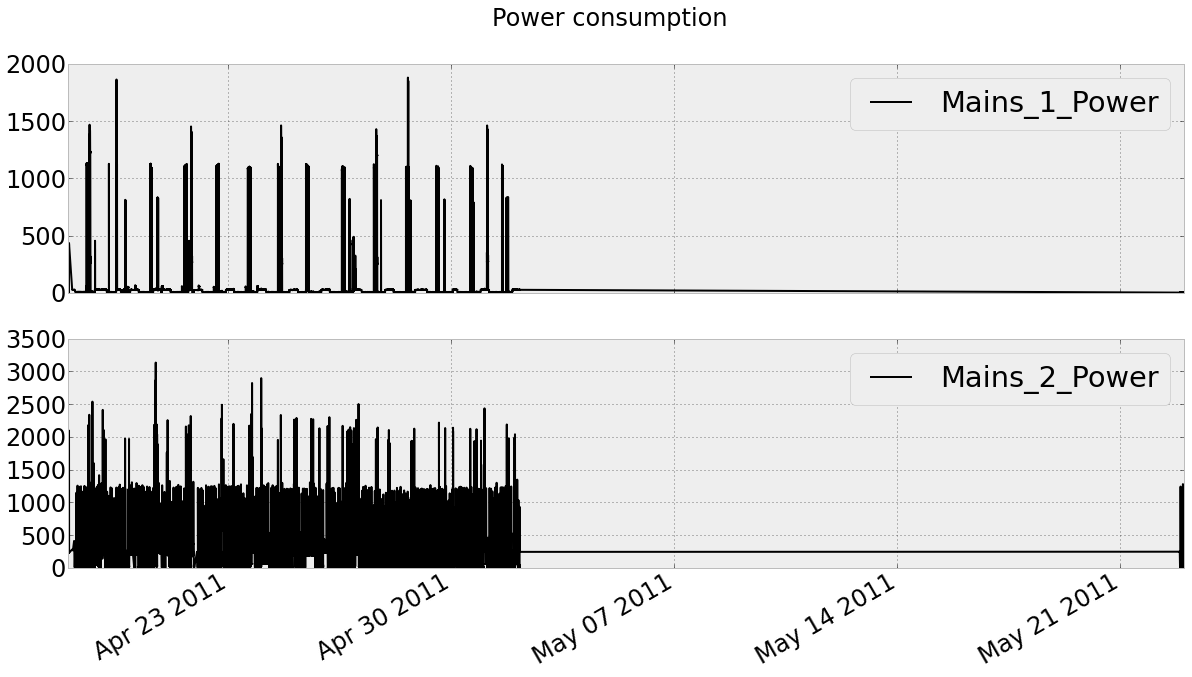
\includegraphics[width=0.7\textwidth]{REDD_House2_Analysis_files/REDD_House2_Analysis_fig_00.png}
\par
\end{center}
\end{codeoutput}
\end{codecell}
This shows an alternative way of plotting using Matplotlib.

\begin{codecell}
\begin{codeinput}
\begin{lstlisting}
plt.title('Mains 1 Power')
plt.xlabel('Time')
plt.ylabel('Power (W)')
plt.figsize(12,7)
matplotlib.rcParams.update({'font.size': 24})
plt.plot(df_mains.index.to_pydatetime(),df_mains.Mains_1_Power)
plt.gca().xaxis.set_major_formatter( DateFormatter('%d\n%b') )
\end{lstlisting}
\end{codeinput}
\begin{codeoutput}
\begin{center}
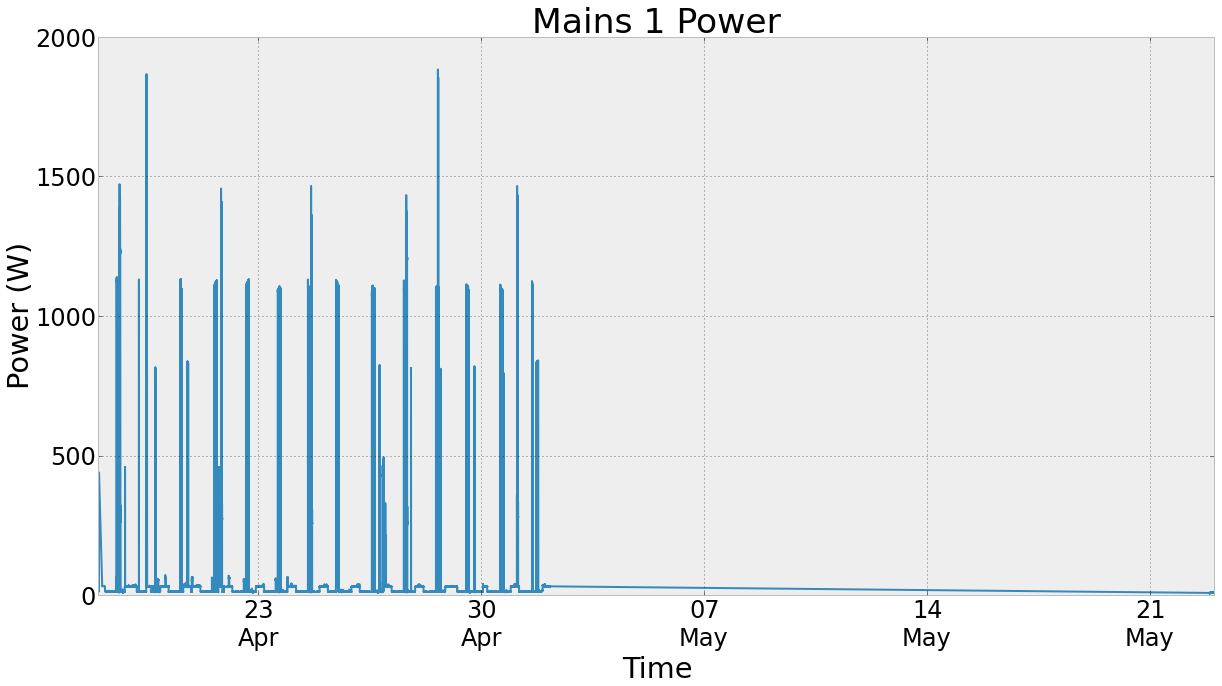
\includegraphics[width=0.7\textwidth]{REDD_House2_Analysis_files/REDD_House2_Analysis_fig_01.png}
\par
\end{center}
\end{codeoutput}
\end{codecell}
\begin{codecell}
\begin{codeinput}
\begin{lstlisting}
plt.title('Mains 2 Power')
plt.xlabel('Time')
plt.ylabel('Power (W)')
plt.figsize(12,7)
matplotlib.rcParams.update({'font.size': 24})
plt.plot(df_mains.index.to_pydatetime(),df_mains.Mains_2_Power)
plt.gca().xaxis.set_major_formatter( DateFormatter('%d\n%b') )
\end{lstlisting}
\end{codeinput}
\begin{codeoutput}
\begin{center}
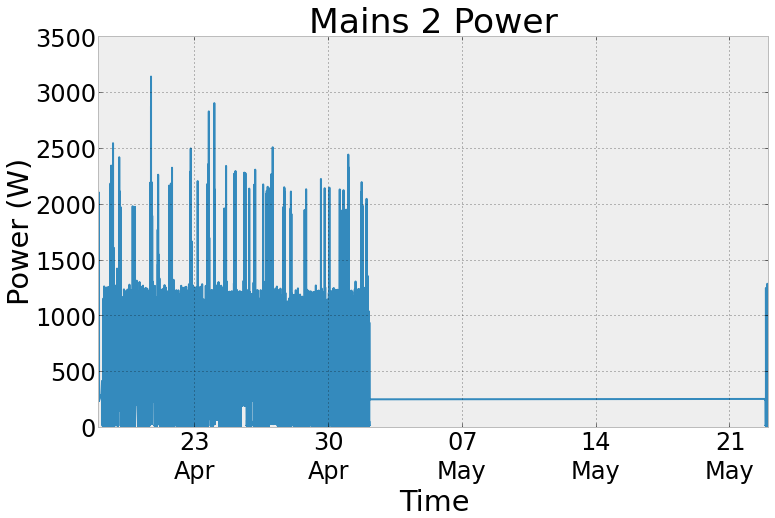
\includegraphics[width=0.7\textwidth]{REDD_House2_Analysis_files/REDD_House2_Analysis_fig_02.png}
\par
\end{center}
\end{codeoutput}
\end{codecell}
Loading appliance data

\begin{codecell}
\begin{codeinput}
\begin{lstlisting}
start_time=time.time()
kitchen_data=np.loadtxt('house_2/channel_3.dat')
light_data=np.loadtxt('house_2/channel_4.dat')
stove_data=np.loadtxt('house_2/channel_5.dat')
microwave_data=np.loadtxt('house_2/channel_6.dat')
washer_dry_data=np.loadtxt('house_2/channel_7.dat')
kitchen_2_data=np.loadtxt('house_2/channel_8.dat')
refrigerator_data=np.loadtxt('house_2/channel_9.dat')
dishwasher_data=np.loadtxt('house_2/channel_10.dat')
disposal_data=np.loadtxt('house_2/channel_11.dat')
kitchen_power=kitchen_data[:,1]
light_power=light_data[:,1]
stove_power=stove_data[:,1]
microwave_power=microwave_data[:,1]
washer_dryer_power=washer_dry_data[:,1]
kitchen_2_power=kitchen_2_data[:,1]
refrigerator_power=refrigerator_data[:,1]
dishwasher_power=dishwasher_data[:,1]
disposal_power=disposal_data[:,1]
timestamp=kitchen_data[:,0]
timestamp_appliance_date=timestamp.astype('datetime64[s]')
end_time=time.time()
print "Time taken to load appliance data= "+str(end_time-start_time)+" seconds"
\end{lstlisting}
\end{codeinput}
\begin{codeoutput}
\begin{verbatim}
Time taken to load appliance data= 27.2005450726 seconds
\end{verbatim}
\end{codeoutput}
\end{codecell}
Creating a data frame of all appliances data

\begin{codecell}
\begin{codeinput}
\begin{lstlisting}
df_appliances=DataFrame({'kitchen':kitchen_power,'light':light_power,'stove':stove_power,'microwave':microwave_power,\
'washer_dryer':washer_dryer_power,'kitchen_2':kitchen_2_power,'refrigerator':refrigerator_power,'dishwasher':dishwasher_power,\
'disposal':disposal_power},index=timestamp_appliance_date)
pd.set_option('display.precision', 2)
print df_appliances.describe().to_string()
\end{lstlisting}
\end{codeinput}
\begin{codeoutput}
\begin{verbatim}
dishwasher  disposal   kitchen  kitchen_2     light  microwave  refrigerator     stove  washer_dryer
count    318759.0  318759.0  318759.0   318759.0  318759.0   318759.0      318759.0  318759.0      318759.0
mean          8.9       0.1       6.2       10.3      26.5       15.3          79.7       1.4           2.1
std          95.7       3.3      37.7       97.4      45.8      110.6          88.0      18.9           0.8
min           0.0       0.0       0.0        0.0       0.0        0.0           0.0       0.0           0.0
25%           0.0       0.0       0.0        1.0       8.0        4.0           6.0       0.0           2.0
50%           0.0       0.0       0.0        1.0       8.0        5.0           7.0       0.0           2.0
75%           0.0       0.0      13.0        1.0       9.0        5.0         161.0       1.0           2.0
max        1457.0     609.0     805.0     1119.0     289.0     1986.0        2246.0     457.0          55.0
\end{verbatim}
\end{codeoutput}
\end{codecell}
\begin{codecell}
\begin{codeinput}
\begin{lstlisting}
df_appliances.refrigerator.plot(rot=0,title='Refrigerator Power')
plt.gca().xaxis.set_major_formatter( DateFormatter('%d\n%b') )
plt.gca().set_ylabel("Power (W)")
plt.gca().set_xlabel("Time");
\end{lstlisting}
\end{codeinput}
\begin{codeoutput}
\begin{center}
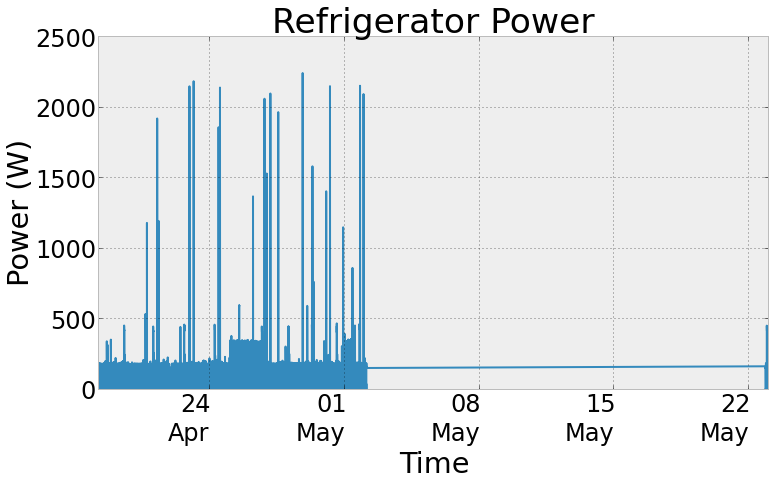
\includegraphics[width=0.7\textwidth]{REDD_House2_Analysis_files/REDD_House2_Analysis_fig_03.png}
\par
\end{center}
\end{codeoutput}
\end{codecell}
Starting time and ending times of channels

\begin{codecell}
\begin{codeinput}
\begin{lstlisting}
print "Mains starting time",df_mains.index[0]
print "Mains ending time",df_mains.index[-1]
print "Mains starting time",df_appliances.index[0]
print "Mains ending time",df_appliances.index[-1]
\end{lstlisting}
\end{codeinput}
\begin{codeoutput}
\begin{verbatim}
Mains starting time 2011-04-17 23:18:27
Mains ending time 2011-05-22 23:59:16
Mains starting time 2011-04-18 05:31:40
Mains ending time 2011-05-22 23:59:08
\end{verbatim}
\end{codeoutput}
\end{codecell}
\subparagraph{Preprocessing}
\begin{codecell}
\begin{codeinput}
\begin{lstlisting}
preprocessed_start_time='04-18-2011 06:00'
preprocessed_end_time='05-01-2011'
df_appliances=df_appliances[preprocessed_start_time:preprocessed_end_time]
df_mains=df_mains[preprocessed_start_time:preprocessed_end_time]
\end{lstlisting}
\end{codeinput}
\end{codecell}
Now plotting

\begin{codecell}
\begin{codeinput}
\begin{lstlisting}
df_mains.plot(subplots=True);
\end{lstlisting}
\end{codeinput}
\begin{codeoutput}
\begin{center}
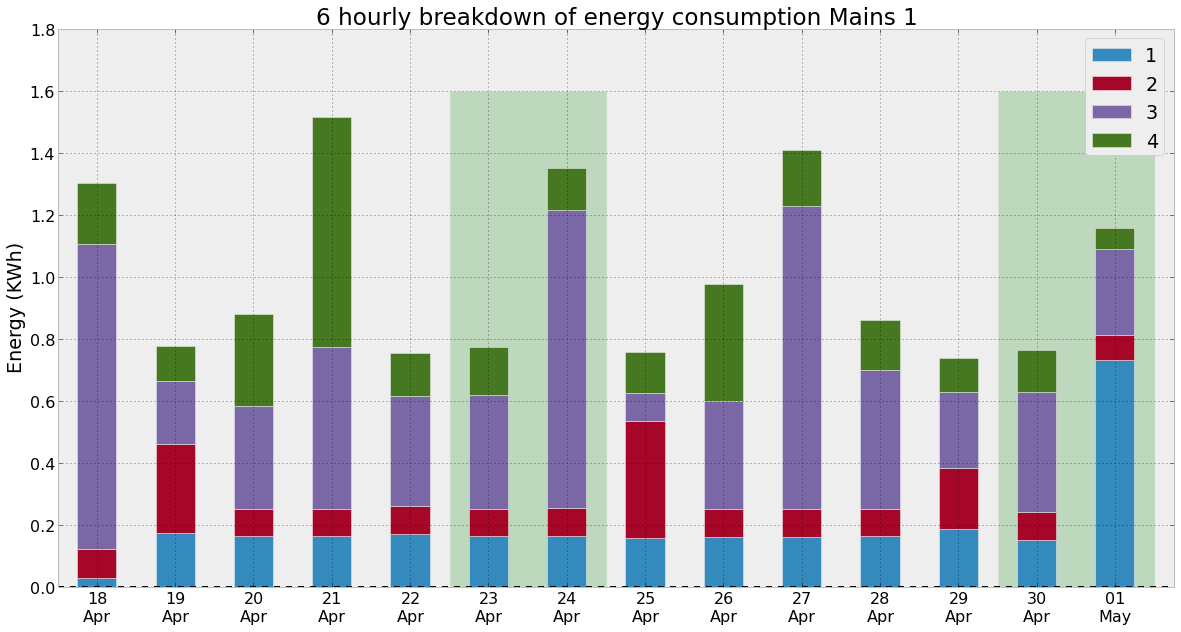
\includegraphics[width=0.7\textwidth]{REDD_House2_Analysis_files/REDD_House2_Analysis_fig_04.png}
\par
\end{center}
\end{codeoutput}
\end{codecell}
\begin{codecell}
\begin{codeinput}
\begin{lstlisting}
df_appliances.refrigerator.plot();
\end{lstlisting}
\end{codeinput}
\begin{codeoutput}
\begin{center}
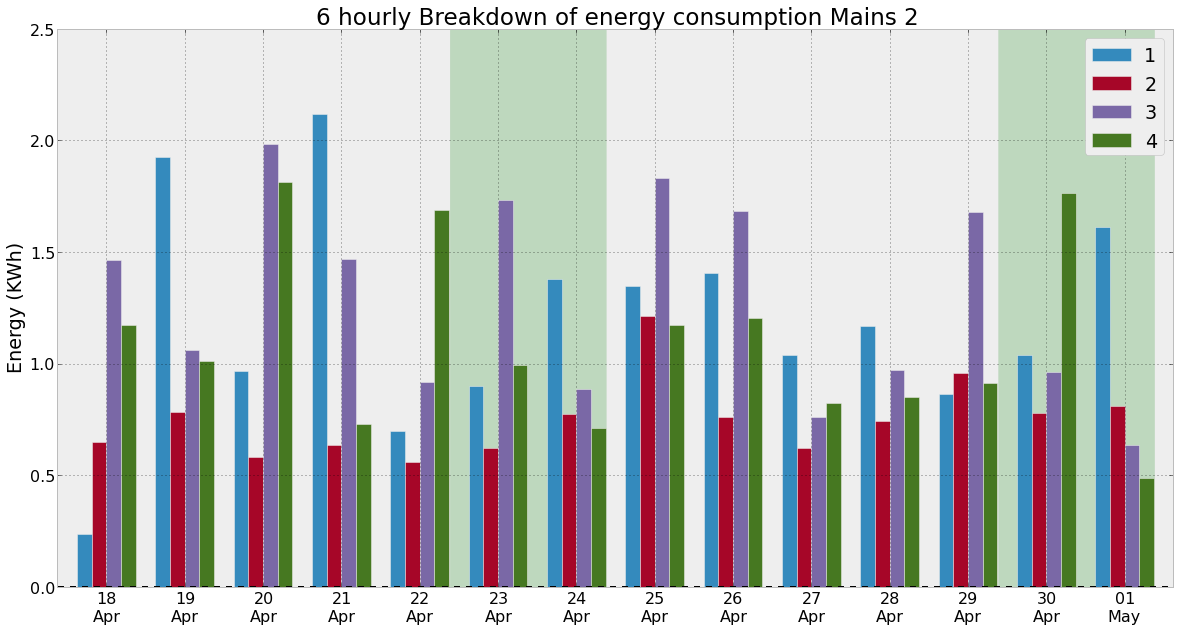
\includegraphics[width=0.7\textwidth]{REDD_House2_Analysis_files/REDD_House2_Analysis_fig_05.png}
\par
\end{center}
\end{codeoutput}
\end{codecell}
\subparagraph{Downsampling Data}
\begin{codecell}
\begin{codeinput}
\begin{lstlisting}
df_appliances_minute=df_appliances.resample('1Min',how='mean')
pd.set_option('display.precision', 2)
print df_appliances_minute.describe().to_string()
\end{lstlisting}
\end{codeinput}
\begin{codeoutput}
\begin{verbatim}
dishwasher  disposal  kitchen  kitchen_2    light  microwave  refrigerator    stove  washer_dryer
count     19580.0   19580.0  19580.0    19580.0  19580.0    19580.0       19580.0  19580.0       19580.0
mean          9.2       0.1      6.2       10.5     26.8       15.5          79.5      1.5           2.2
std          96.0       1.6     34.9       74.1     46.0       97.2          85.4     18.0           0.6
min           0.0       0.0      0.0        0.0      2.0        1.6           1.6      0.0           0.0
25%           0.0       0.0      0.0        1.0      8.0        4.1           6.1      0.1           2.0
50%           0.1       0.0      0.4        1.0      8.6        4.6           7.0      0.5           2.0
75%           0.1       0.0     13.0        1.0      9.0        5.0         160.7      0.9           2.2
max        1255.6     115.8    794.6     1071.8    185.4     1926.0         598.2    411.0           8.8
\end{verbatim}
\end{codeoutput}
\end{codecell}
\begin{codecell}
\begin{codeinput}
\begin{lstlisting}
df_mains_minute=df_mains.resample('1Min',how='mean')
df_mains_minute.describe()
\end{lstlisting}
\end{codeinput}
\begin{codeoutput}
\begin{verbatim}
       Mains_1_Power  Mains_2_Power
count        19579.0        19579.0
mean            43.4          188.2
std            129.8          206.7
min             13.4           21.4
25%             14.9           22.5
50%             15.1          214.1
75%             33.7          259.1
max           1312.0         2612.5
\end{verbatim}
\end{codeoutput}
\end{codecell}
As a sanity check, we confirm that 19400 minutes correspond to about 14
days, thus our resampling was correct. We next align mains and appliance
time series.

\subparagraph{Filling  Missing Data with forward filling}
\begin{codecell}
\begin{codeinput}
\begin{lstlisting}
print "Number of missing values in Mains",sum(pd.isnull(df_mains_minute.Mains_1_Power))
print "Number of missing values in Appliances",sum(pd.isnull(df_appliances_minute.refrigerator))
\end{lstlisting}
\end{codeinput}
\begin{codeoutput}
\begin{verbatim}
Number of missing values in Mains 221
Number of missing values in Appliances 220
\end{verbatim}
\end{codeoutput}
\end{codecell}
\begin{codecell}
\begin{codeinput}
\begin{lstlisting}
df_appliances_minute.fillna(method='pad',inplace=True)
df_mains_minute.fillna(method='pad',inplace=True)
assert 0==sum(pd.isnull(df_mains_minute.Mains_1_Power))
assert 0==sum(pd.isnull(df_appliances_minute.refrigerator))
\end{lstlisting}
\end{codeinput}
\end{codecell}
\subparagraph{Finding contributions of different appliances and discarding loads with insignificant contribution}
\begin{codecell}
\begin{codeinput}
\begin{lstlisting}
total_power=np.sum(df_mains_minute.Mains_1_Power.values+df_mains_minute.Mains_2_Power.values)
for appliance in df_appliances_minute:
    print "Contribution of %s to overall load is %f" %(appliance,100*np.sum(df_appliances_minute[appliance].values)/total_power)
\end{lstlisting}
\end{codeinput}
\begin{codeoutput}
\begin{verbatim}
Contribution of dishwasher to overall load is 3.918053
Contribution of disposal to overall load is 0.035672
Contribution of kitchen to overall load is 2.706929
Contribution of kitchen_2 to overall load is 4.484684
Contribution of light to overall load is 11.694800
Contribution of microwave to overall load is 6.645737
Contribution of refrigerator to overall load is 34.357508
Contribution of stove to overall load is 0.630176
Contribution of washer_dryer to overall load is 0.933156
\end{verbatim}
\end{codeoutput}
\end{codecell}
Since washer dryer has a peak usage of 8 W, we assume that to be noise
in the circuit. Also, disposal has usage of less than .1 \% and is thus
not further included in the analysis. EVen though stove has less than
0.1 \% contribution, it has few instances of being used in high power
mode.

\subparagraph{Sorting appliances in decreasing order of peak power consumption}
Creating a dictionary of the form \{appliance: peak power\} and then
sorting it by value

\begin{codecell}
\begin{codeinput}
\begin{lstlisting}
appliance_peak_power_dict={}
for appliance in df_appliances_minute:
    if appliance not in ['washer_dryer','disposal']:
        appliance_peak_power_dict[appliance]=df_appliances_minute[appliance].max()
#This variable is named 's' in the algorithm described in the paper
sorted_appliance_list=sorted(appliance_peak_power_dict, key=appliance_peak_power_dict.get, reverse=True)
\end{lstlisting}
\end{codeinput}
\end{codecell}
\subparagraph{Load Assignment to Mains}
\begin{codecell}
\begin{codeinput}
\begin{lstlisting}
mapping={}
df_mains_minute_copy=df_mains_minute.copy()
converged=False
\end{lstlisting}
\end{codeinput}
\end{codecell}
\begin{codecell}
\begin{codeinput}
\begin{lstlisting}
df_mains_minute_copy=df_mains_minute.copy()
converged=False
mapping={}
def thresholding_based_load_assignment(mapping,sorted_appliance_list,converged,TOLERANCE):
    iteration=-1
    while converged==False:
        before_iteration_len_mapping=len(mapping.keys())
        iteration+=1
        for load in sorted_appliance_list:
            if load not in mapping:
                #Since mains 1 has less average load we check it first
                #Note we may need some tolerance as 1-2 values may be off, but more than 20 odd values satisying
                #would mean that we can safely assign the other mains
                
                c1=len(np.where((df_appliances_minute[load].values-df_mains_minute_copy.Mains_1_Power.values)>0)[0])
                c2=len(np.where((df_appliances_minute[load].values-df_mains_minute_copy.Mains_2_Power.values)>0)[0])
                #Using a copy of the Mains Minute DF rather than the original 
                
                if c1>TOLERANCE and c2<TOLERANCE:       
                    mapping[load]=2
                elif c2>TOLERANCE and c1<TOLERANCE:
                    mapping[load]=1
            
                #Subtracting Load from the assigned Mains and filling in zeros for 
                #few spots where appliance value might be more due to error
            if load in mapping:
                #Load has been assined
                if mapping[load]==1:
                    df_mains_minute_copy.Mains_1_Power=df_mains_minute_copy.Mains_1_Power-df_appliances_minute[load]
                    df_mains_minute_copy.Mains_1_Power[df_mains_minute_copy.Mains_1_Power<0]=0
                else:
                    df_mains_minute_copy.Mains_2_Power=df_mains_minute_copy.Mains_2_Power-df_appliances_minute[load]
                    df_mains_minute_copy.Mains_2_Power[df_mains_minute_copy.Mains_2_Power<0]=0
      
        print "After iteration %d" %iteration
        print mapping
        after_iteration_len_mapping=len(mapping.keys())
        if after_iteration_len_mapping==before_iteration_len_mapping:
            converged=True            
\end{lstlisting}
\end{codeinput}
\end{codecell}
\begin{codecell}
\begin{codeinput}
\begin{lstlisting}
thresholding_based_load_assignment(mapping,sorted_appliance_list,False,300)
\end{lstlisting}
\end{codeinput}
\begin{codeoutput}
\begin{verbatim}
After iteration 0
{'refrigerator': 2, 'light': 2, 'kitchen_2': 1, 'microwave': 2}
After iteration 1
{'refrigerator': 2, 'light': 2, 'dishwasher': 1, 'kitchen_2': 1, 'microwave': 2}
After iteration 2
{'refrigerator': 2, 'light': 2, 'dishwasher': 1, 'kitchen_2': 1, 'microwave': 2}
\end{verbatim}
\end{codeoutput}
\end{codecell}
Now we need to find according to step change the load assignment

Only `kitchen' and `stove' have not yet been separated into mains.
Finding step changes of more than 15 W threshold in these loads and
seeing the times at which these step changes take place.

\begin{codecell}
\begin{codeinput}
\begin{lstlisting}
def step_changes(series,threshold):
    diff_series=np.diff(series.values)
    print diff_series
    return {"magnitude":diff_series,"times":series[np.abs(diff_series)>threshold].index}
    #Finding times at which these step changes take place
    
\end{lstlisting}
\end{codeinput}
\end{codecell}
\begin{codecell}
\begin{codeinput}
\begin{lstlisting}
step_threshold=30
for load in sorted_appliance_list:
    if load not in mapping:
        
        step_load=set(step_changes(df_appliances_minute[load],step_threshold)["times"]);
        step_mains_1=set(step_changes(df_mains_minute.Mains_1_Power,step_threshold)["times"]);
        step_mains_2=set(step_changes(df_mains_minute.Mains_2_Power,step_threshold)["times"]);
        
        #Find intersection with Mains 1 and 2
        l1=len(step_load.intersection(step_mains_1));
        l2=len(step_load.intersection(step_mains_2));
        
        if 1.0*l1/len(step_load)>0.9:
            #More than 90% events detected
            mapping[load]=1
        elif 1.0*l2/len(step_load)>0.9:
            #More than 90% events detected
            mapping[load]=2
        else:
            print "Load could not be assigned"       
      
\end{lstlisting}
\end{codeinput}
\end{codecell}
\begin{codecell}
\begin{codeinput}
\begin{lstlisting}
print "Appliance to Mains Mapping\n"
pprint.pprint(mapping)
\end{lstlisting}
\end{codeinput}
\begin{codeoutput}
\begin{verbatim}
Appliance to Mains Mapping

{'dishwasher': 1,
 'kitchen': 1,
 'kitchen_2': 1,
 'light': 2,
 'microwave': 2,
 'refrigerator': 2,
 'stove': 1}
\end{verbatim}
\end{codeoutput}
\end{codecell}
\subparagraph{Dividing Data into TEST and TRAIN}
\begin{codecell}
\begin{codeinput}
\begin{lstlisting}
df_mains_train=df_mains_minute[:'2011-4-24']
df_mains_test=df_mains_minute['2011-4-25':]
df_appliances_train=df_appliances_minute[:'2011-4-24']
df_appliances_test=df_appliances_minute['2011-4-25':]
\end{lstlisting}
\end{codeinput}
\end{codecell}
\subparagraph{Perform KMeans++ and Mini Batch KMeans on Train set}
\begin{codecell}
\begin{codeinput}
\begin{lstlisting}

plt.figsize(15,8)
matplotlib.rcParams.update({'font.size': 24})
\end{lstlisting}
\end{codeinput}
\end{codecell}
Reshaping data so that it can be used by clustering algos

\begin{codecell}
\begin{codeinput}
\begin{lstlisting}
raw_data={}
for key in df_appliances_train:
    raw_data[key]=df_appliances_train[key].values
    length=len(raw_data[key])
    raw_data[key]=raw_data[key].reshape(length,1)
centroids={}
\end{lstlisting}
\end{codeinput}
\end{codecell}
\begin{codecell}
\begin{codeinput}
\begin{lstlisting}
batch_size=1000
def apply_kmeans(n_clusters, n_init,X,init=None):
    matplotlib.rcParams.update({'font.size': 16})
    if init is None:
        k_means = KMeans(n_clusters=n_clusters, n_init=n_init)
    else:
        k_means=KMeans(init='k-means++',n_clusters=n_clusters, n_init=n_init)
    t0 = time.time()
    k_means.fit(X)
    t_batch = time.time() - t0
    k_means_labels = k_means.labels_
    k_means_cluster_centers = k_means.cluster_centers_
    k_means_labels_unique = np.unique(k_means_labels)
    k_means_inertia=k_means.inertia_
    mbk = MiniBatchKMeans(init='k-means++', n_clusters=n_clusters, batch_size=batch_size,
                      n_init=n_init, max_no_improvement=10, verbose=0)
    t0 = time.time()
    mbk.fit(X)
    t_mini_batch = time.time() - t0
    mbk_means_labels = mbk.labels_
    mbk_means_cluster_centers = mbk.cluster_centers_
    mbk_means_labels_unique = np.unique(mbk_means_labels)
    mbk_inertia=mbk.inertia_
    return [t_batch, t_mini_batch, k_means_labels, mbk_means_labels, k_means_cluster_centers, mbk_means_cluster_centers,\
    k_means_labels_unique,mbk_means_labels_unique, k_means_inertia, mbk_inertia] 
\end{lstlisting}
\end{codeinput}
\end{codecell}
\begin{codecell}
\begin{codeinput}
\begin{lstlisting}
def plot_cluster_assignments(X,k_means_labels, mbk_means_labels,k_means_cluster_centers,mbk_means_cluster_centers,n_clusters,appliance_name):
    colors = ['#4EACC5', '#FF9C34', '#4E9A06']
    markers=['o','*','.']
    x_temp=np.arange(len(X))
    plt.subplot(2,2,1)
    #plt.rcParams["font.size"]=16
    print "\nKMeans Analysis for %s\n" %appliance_name
    print "-"*80
    centroids[appliance_name]=[]
    for k, col in zip(range(n_clusters), colors):
        my_members = k_means_labels == k
        cluster_center = k_means_cluster_centers[k]    
        centroids[appliance_name].append(k_means_cluster_centers[k][0])
        plt.ylabel('Power (W)');
        plt.plot(x_temp[my_members],X[my_members, 0],markers[k],markersize=20,markerfacecolor=col) 
        plt.axhline(k_means_cluster_centers[k],linewidth=6,color=col)
        print "State %d Centroid= %0.4f, Fraction of datapoints= %0.4f" %(k,cluster_center,sum(my_members)*1.0/np.size(X))
        plt.title('KMeans Cluster Assignment for '+appliance_name+' for K='+str(n_clusters))
        plt.xlabel("Samples")
    plt.subplot(2,2,2)
    plt.tight_layout()
    print "\nMini Batch KMeans Analysis\n"
    print "-"*80
    for k, col in zip(range(n_clusters), colors):
        my_members = mbk_means_labels == k
        cluster_center = mbk_means_cluster_centers[k]    
        plt.ylabel('Power (W)');
        plt.plot(x_temp[my_members],X[my_members, 0],markers[k],markersize=15,markerfacecolor=col) 
        plt.axhline(mbk_means_cluster_centers[k],linewidth=3,color=col)
        print "State %d Centroid= %0.4f, Fraction of datapoints= %0.4f" %(k,cluster_center,sum(my_members)*1.0/np.size(X))
        #plt.title('Mini Batch KMeans Cluster Assignment for '+appliance_name+' for K='+str(n_clusters))
    print "-"*80
    
\end{lstlisting}
\end{codeinput}
\end{codecell}
Peforming clustering for different appliance. \textbf{Caveat}: Number of
states must be known beforehand

\begin{codecell}
\begin{codeinput}
\begin{lstlisting}
appliances_mains=[[],[]]
appliances_states=[[3,2,3,2],[3,3,3]]
appliances_mains[0]=[key for key in mapping if mapping[key]==1] 
appliances_mains[1]=[key for key in mapping if mapping[key]==2]
labels_appliance={}

\end{lstlisting}
\end{codeinput}
\end{codecell}
\begin{codecell}
\begin{codeinput}
\begin{lstlisting}
for i in range(len(appliances_mains[0])):
    figure()
    [t_batch, t_mini_batch, k_means_labels, mbk_means_labels, k_means_cluster_centers, mbk_means_cluster_centers,\
    k_means_labels_unique,mbk_means_labels_unique, k_means_inertia, mbk_inertia]=apply_kmeans(appliances_states[0][i],10,raw_data[appliances_mains[0][i]],"kmeans++")
    plot_cluster_assignments(raw_data[appliances_mains[0][i]],k_means_labels, mbk_means_labels, k_means_cluster_centers, mbk_means_cluster_centers\
    ,appliances_states[0][i],appliances_mains[0][i])
    print "Time taken for Kmeans clustering    :     \n",t_batch
    print "Inertia of KMeans cluster assignment:     \n",k_means_inertia
    print "Time taken for Mini Batch Kmeans clustering    :     \n",t_mini_batch
    print "Inertia of Mini Batch KMeans cluster assignment:     \n",mbk_inertia
    flattened=k_means_cluster_centers.flatten()
    sorted_list=sort(flattened)
    labels=[]
    for label in k_means_labels:
        labels.append(sorted_list.tolist().index(flattened[label]))
    labels_appliance[appliances_mains[0][i]]=np.array(labels)
\end{lstlisting}
\end{codeinput}
\begin{codeoutput}
\begin{verbatim}
KMeans Analysis for dishwasher

--------------------------------------------------------------------------------
State 0 Centroid= 0.1701, Fraction of datapoints= 0.9849
State 1 Centroid= 1195.3714, Fraction of datapoints= 0.0074
State 2 Centroid= 260.5342, Fraction of datapoints= 0.0077

Mini Batch KMeans Analysis
\end{verbatim}
\begin{verbatim}
--------------------------------------------------------------------------------
State 0 Centroid= 0.1740, Fraction of datapoints= 0.9849
State 1 Centroid= 1195.3284, Fraction of datapoints= 0.0074
State 2 Centroid= 259.3460, Fraction of datapoints= 0.0077
--------------------------------------------------------------------------------
Time taken for Kmeans clustering    :     
0.0920648574829
Inertia of KMeans cluster assignment:     
817407.717216
Time taken for Mini Batch Kmeans clustering    :     
0.0314409732819
Inertia of Mini Batch KMeans cluster assignment:     
817513.868037

KMeans Analysis for stove
\end{verbatim}
\begin{verbatim}
--------------------------------------------------------------------------------
State 0 Centroid= 0.6031, Fraction of datapoints= 0.9977
State 1 Centroid= 373.8506, Fraction of datapoints= 0.0023

Mini Batch KMeans Analysis
\end{verbatim}
\begin{verbatim}
--------------------------------------------------------------------------------
State 0 Centroid= 0.5882, Fraction of datapoints= 0.9977
State 1 Centroid= 358.8860, Fraction of datapoints= 0.0023
--------------------------------------------------------------------------------
Time taken for Kmeans clustering    :     
0.0335509777069
Inertia of KMeans cluster assignment:     
159053.555617
Time taken for Mini Batch Kmeans clustering    :     
0.0228269100189
Inertia of Mini Batch KMeans cluster assignment:     
163982.339231

KMeans Analysis for kitchen_2
\end{verbatim}
\begin{verbatim}
--------------------------------------------------------------------------------
State 0 Centroid= 1.4256, Fraction of datapoints= 0.9737
State 1 Centroid= 1036.0541, Fraction of datapoints= 0.0044
State 2 Centroid= 204.7067, Fraction of datapoints= 0.0219

Mini Batch KMeans Analysis
\end{verbatim}
\begin{verbatim}
--------------------------------------------------------------------------------
State 0 Centroid= 1.3737, Fraction of datapoints= 0.9737
State 1 Centroid= 1033.3184, Fraction of datapoints= 0.0044
State 2 Centroid= 205.0644, Fraction of datapoints= 0.0219
--------------------------------------------------------------------------------
Time taken for Kmeans clustering    :     
0.0453970432281
Inertia of KMeans cluster assignment:     
1298012.8041
Time taken for Mini Batch Kmeans clustering    :     
0.0339980125427
Inertia of Mini Batch KMeans cluster assignment:     
1298387.36148

KMeans Analysis for kitchen
\end{verbatim}
\begin{verbatim}
--------------------------------------------------------------------------------
State 0 Centroid= 5.0766, Fraction of datapoints= 0.9987
State 1 Centroid= 727.4287, Fraction of datapoints= 0.0013

Mini Batch KMeans Analysis
\end{verbatim}
\begin{verbatim}
--------------------------------------------------------------------------------
State 0 Centroid= 4.9849, Fraction of datapoints= 0.9987
State 1 Centroid= 731.3755, Fraction of datapoints= 0.0013
--------------------------------------------------------------------------------
Time taken for Kmeans clustering    :     
0.0318310260773
Inertia of KMeans cluster assignment:     
875870.13267
Time taken for Mini Batch Kmeans clustering    :     
0.029895067215
Inertia of Mini Batch KMeans cluster assignment:     
876154.225538
\end{verbatim}
\begin{center}
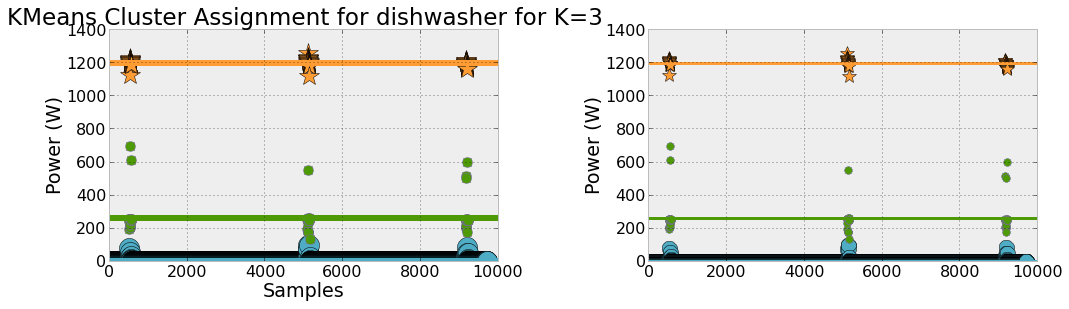
\includegraphics[width=0.7\textwidth]{REDD_House2_Analysis_files/REDD_House2_Analysis_fig_06.png}
\par
\end{center}
\begin{center}
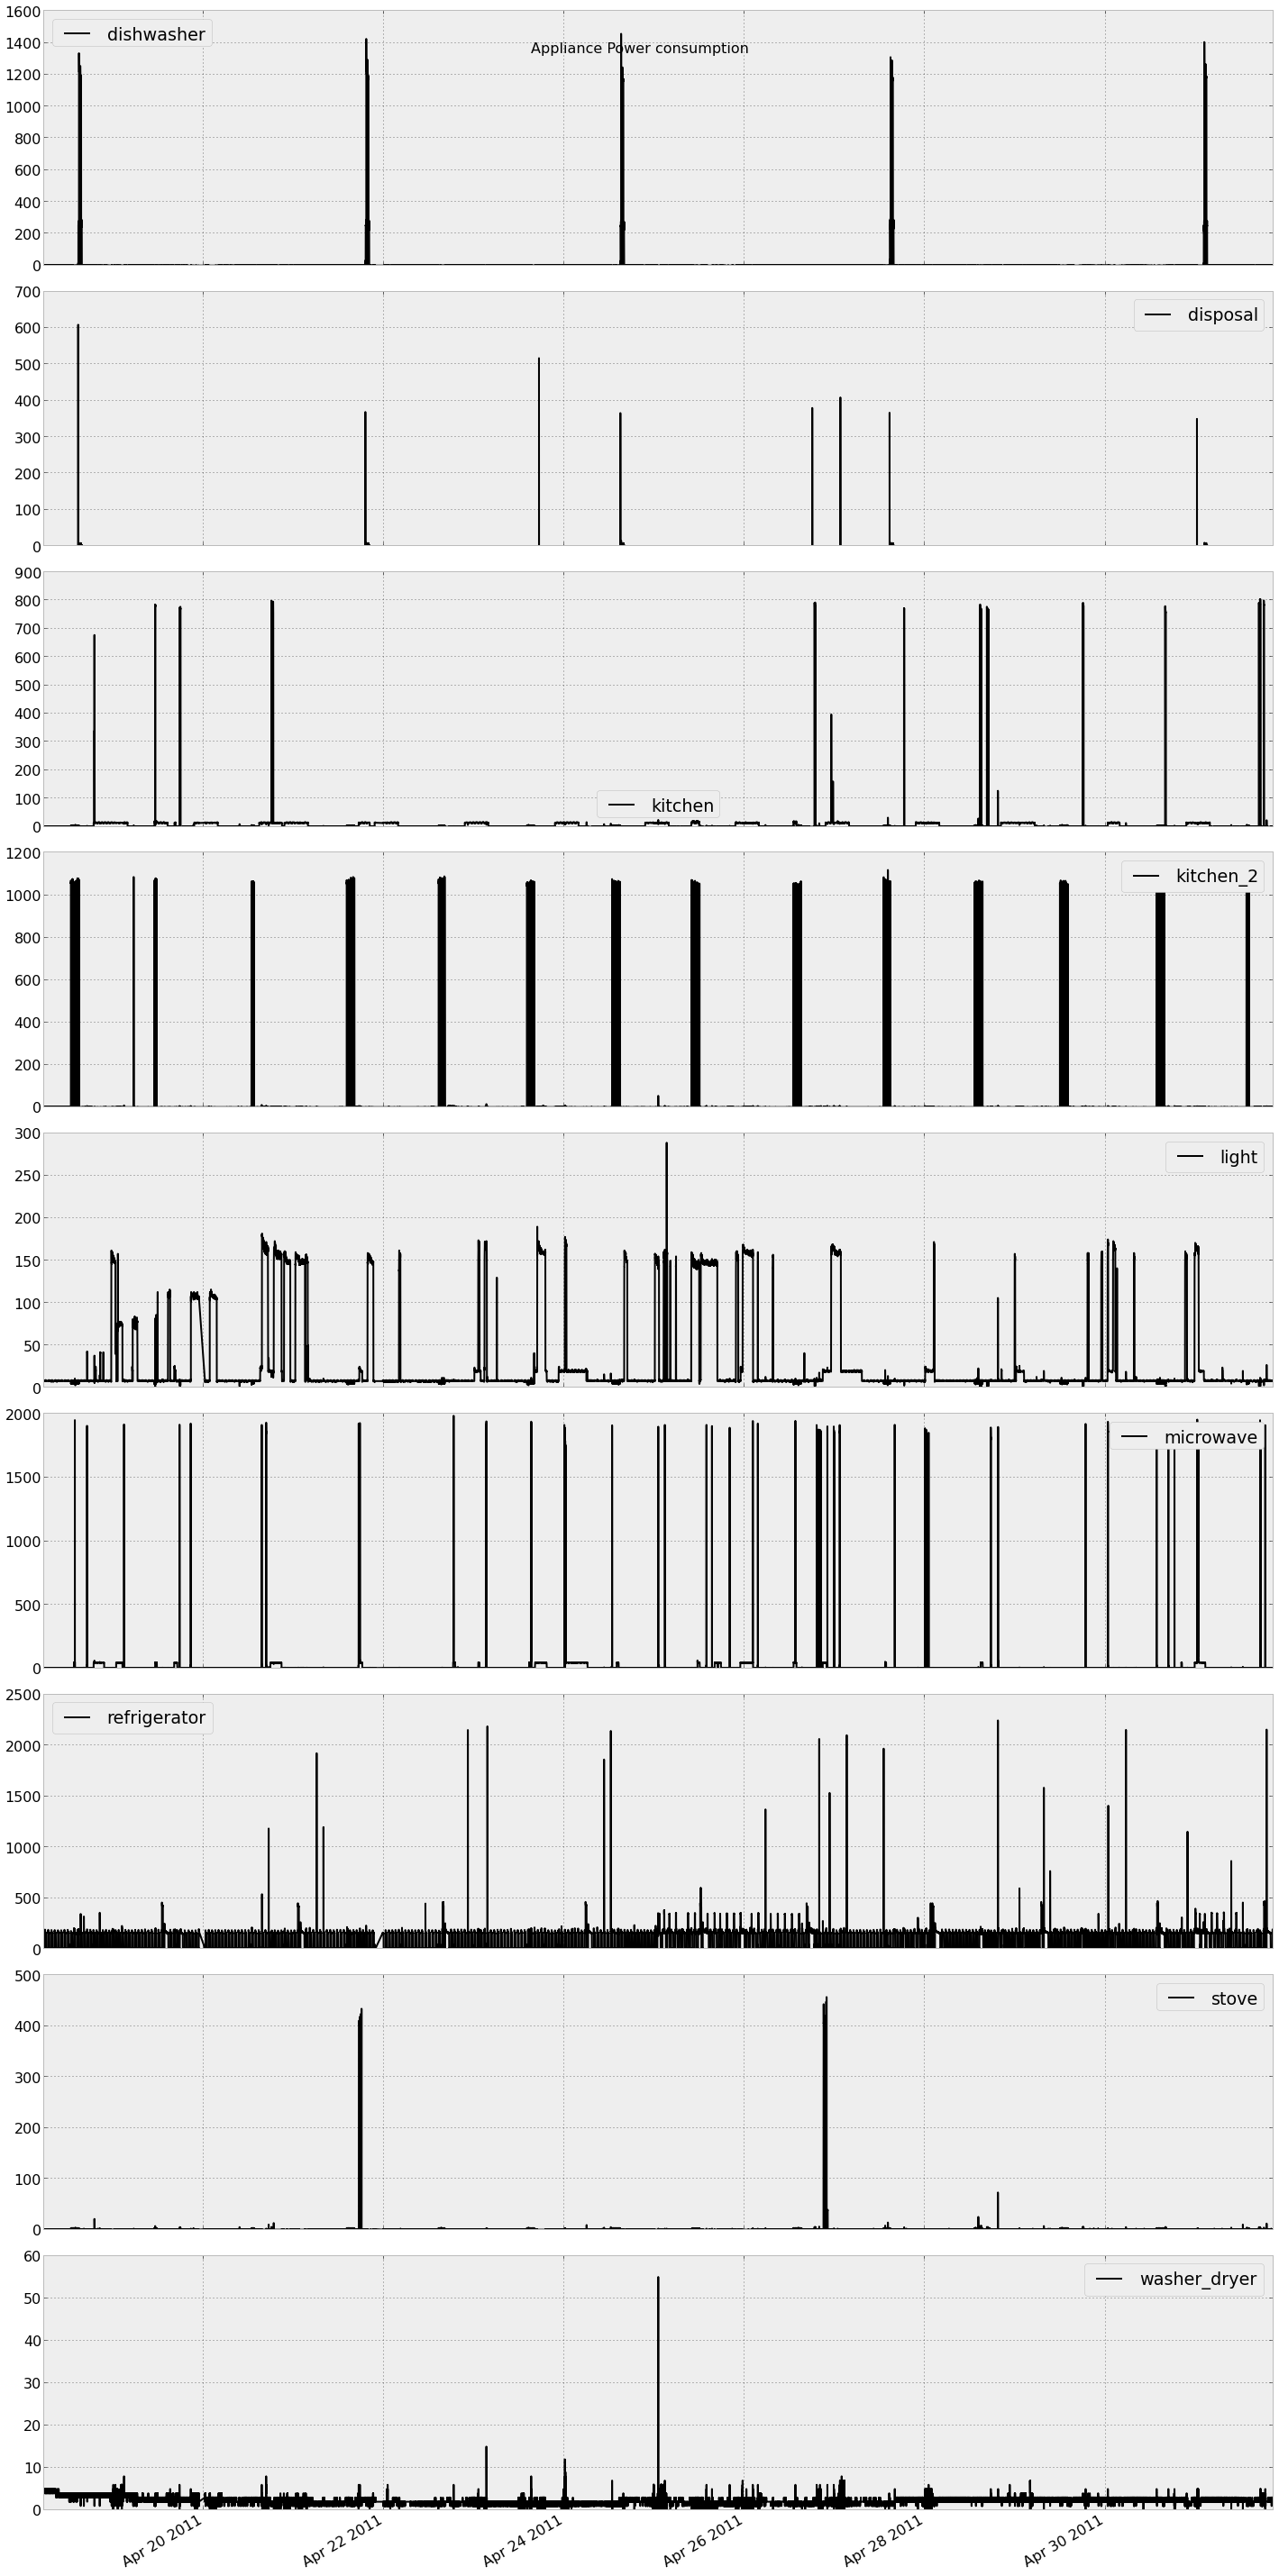
\includegraphics[width=0.7\textwidth]{REDD_House2_Analysis_files/REDD_House2_Analysis_fig_07.png}
\par
\end{center}
\begin{center}
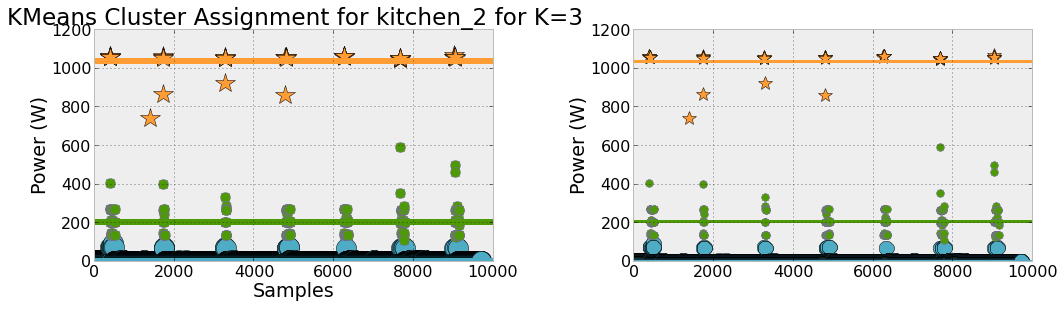
\includegraphics[width=0.7\textwidth]{REDD_House2_Analysis_files/REDD_House2_Analysis_fig_08.png}
\par
\end{center}
\begin{center}
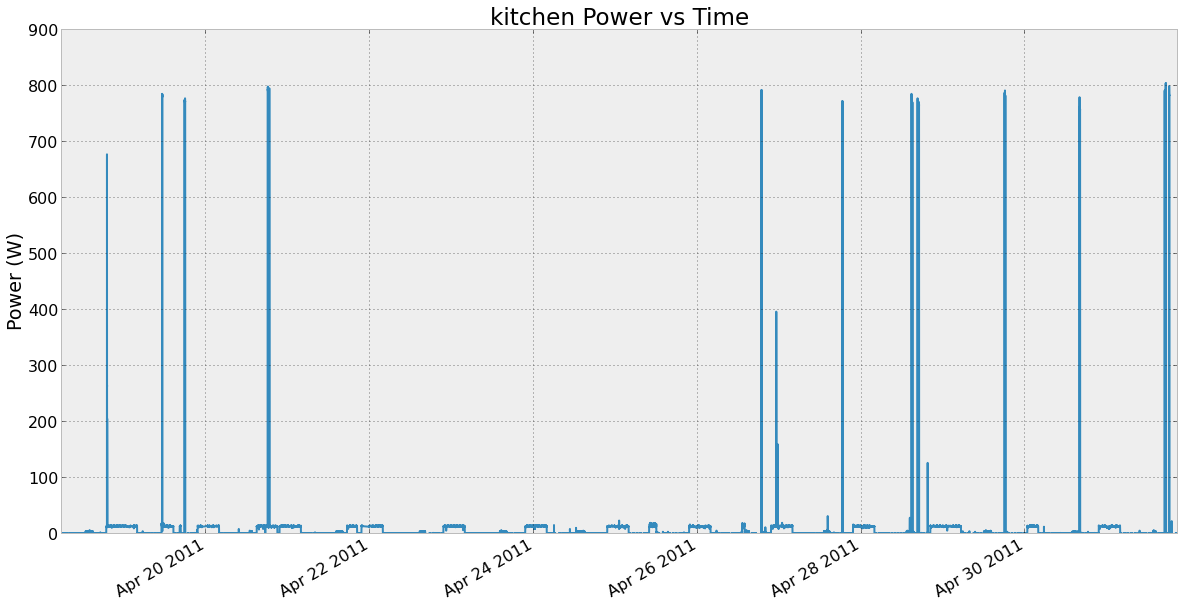
\includegraphics[width=0.7\textwidth]{REDD_House2_Analysis_files/REDD_House2_Analysis_fig_09.png}
\par
\end{center}
\end{codeoutput}
\end{codecell}
\begin{codecell}
\begin{codeinput}
\begin{lstlisting}
for i in range(len(appliances_mains[1])):
    figure()
    [t_batch, t_mini_batch, k_means_labels, mbk_means_labels, k_means_cluster_centers, mbk_means_cluster_centers,\
    k_means_labels_unique,mbk_means_labels_unique, k_means_inertia, mbk_inertia]=apply_kmeans(appliances_states[1][i],10,raw_data[appliances_mains[1][i]],"kmeans++")
    plot_cluster_assignments(raw_data[appliances_mains[1][i]],k_means_labels, mbk_means_labels, k_means_cluster_centers, mbk_means_cluster_centers\
    ,appliances_states[1][i],appliances_mains[1][i])
    print "Time taken for Kmeans clustering    :     \n",t_batch
    print "Inertia of KMeans cluster assignment:     \n",k_means_inertia
    print "Time taken for Mini Batch Kmeans clustering    :     \n",t_mini_batch
    print "Inertia of Mini Batch KMeans cluster assignment:     \n",mbk_inertia
    flattened=k_means_cluster_centers.flatten()
    sorted_list=sort(flattened)
    labels=[]
    for label in k_means_labels:
        labels.append(sorted_list.tolist().index(flattened[label]))
    labels_appliance[appliances_mains[1][i]]=np.array(labels)
\end{lstlisting}
\end{codeinput}
\begin{codeoutput}
\begin{verbatim}
KMeans Analysis for light

--------------------------------------------------------------------------------
State 0 Centroid= 9.4713, Fraction of datapoints= 0.8435
State 1 Centroid= 156.3087, Fraction of datapoints= 0.0987
State 2 Centroid= 96.8437, Fraction of datapoints= 0.0578

Mini Batch KMeans Analysis
\end{verbatim}
\begin{verbatim}
--------------------------------------------------------------------------------
State 0 Centroid= 9.4884, Fraction of datapoints= 0.8435
State 1 Centroid= 156.3094, Fraction of datapoints= 0.0987
State 2 Centroid= 96.5191, Fraction of datapoints= 0.0578
--------------------------------------------------------------------------------
Time taken for Kmeans clustering    :     
0.0435490608215
Inertia of KMeans cluster assignment:     
316625.182718
Time taken for Mini Batch Kmeans clustering    :     
0.032781124115
Inertia of Mini Batch KMeans cluster assignment:     
316686.830452

KMeans Analysis for microwave
\end{verbatim}
\begin{verbatim}
--------------------------------------------------------------------------------
State 0 Centroid= 9.7742, Fraction of datapoints= 0.9966
State 1 Centroid= 1740.2292, Fraction of datapoints= 0.0014
State 2 Centroid= 822.5147, Fraction of datapoints= 0.0020

Mini Batch KMeans Analysis
\end{verbatim}
\begin{verbatim}
--------------------------------------------------------------------------------
State 0 Centroid= 9.7347, Fraction of datapoints= 0.9966
State 1 Centroid= 1751.7149, Fraction of datapoints= 0.0014
State 2 Centroid= 835.3426, Fraction of datapoints= 0.0020
--------------------------------------------------------------------------------
Time taken for Kmeans clustering    :     
0.0832650661469
Inertia of KMeans cluster assignment:     
3282726.04781
Time taken for Mini Batch Kmeans clustering    :     
0.0298271179199
Inertia of Mini Batch KMeans cluster assignment:     
3287714.57283

KMeans Analysis for refrigerator
\end{verbatim}
\begin{verbatim}
--------------------------------------------------------------------------------
State 0 Centroid= 161.8361, Fraction of datapoints= 0.3856
State 1 Centroid= 7.4547, Fraction of datapoints= 0.6079
State 2 Centroid= 423.5390, Fraction of datapoints= 0.0065

Mini Batch KMeans Analysis
\end{verbatim}
\begin{verbatim}
--------------------------------------------------------------------------------
State 0 Centroid= 7.4990, Fraction of datapoints= 0.6078
State 1 Centroid= 161.6750, Fraction of datapoints= 0.3857
State 2 Centroid= 425.9683, Fraction of datapoints= 0.0065
--------------------------------------------------------------------------------
Time taken for Kmeans clustering    :     
0.0451371669769
Inertia of KMeans cluster assignment:     
864286.317816
Time taken for Mini Batch Kmeans clustering    :     
0.0412509441376
Inertia of Mini Batch KMeans cluster assignment:     
864752.643469
\end{verbatim}
\begin{center}
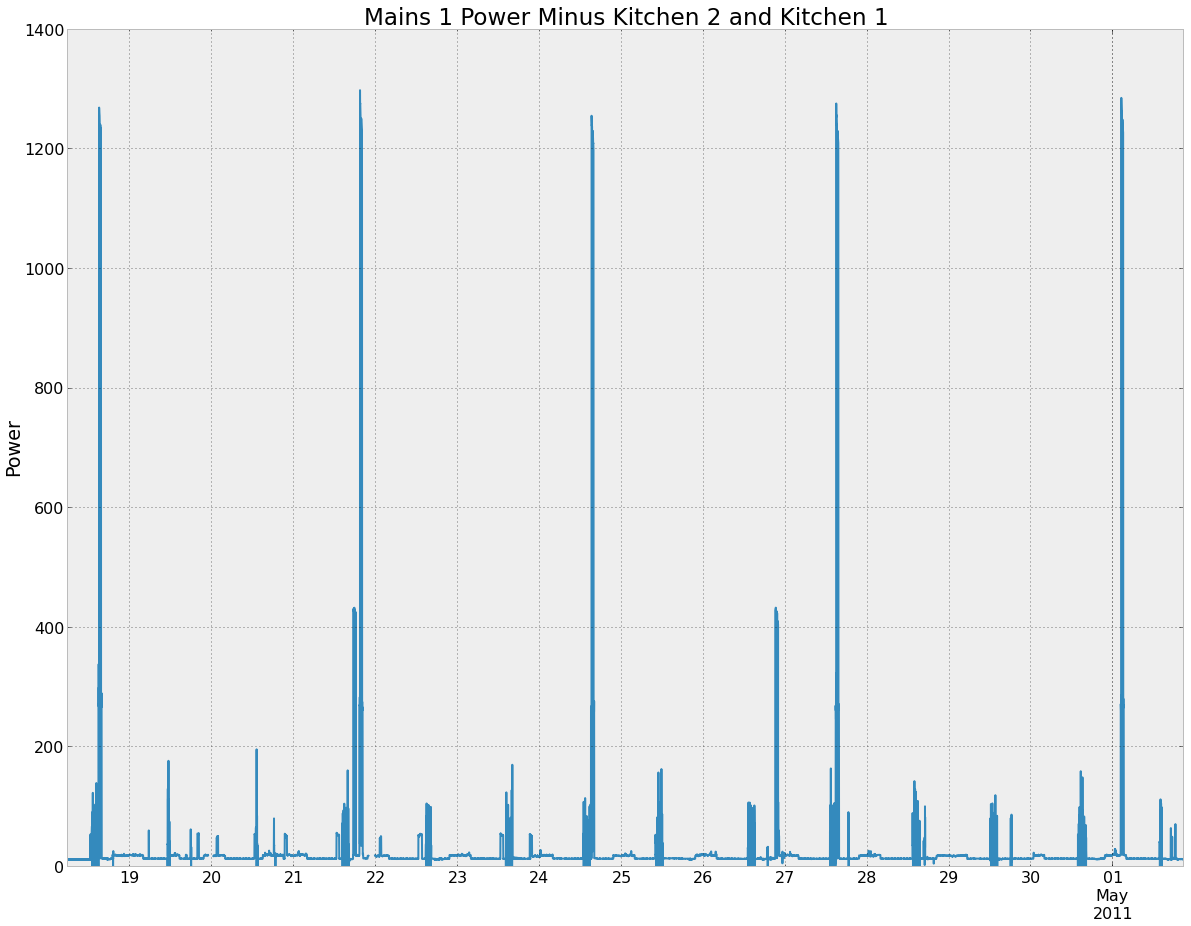
\includegraphics[width=0.7\textwidth]{REDD_House2_Analysis_files/REDD_House2_Analysis_fig_10.png}
\par
\end{center}
\begin{center}
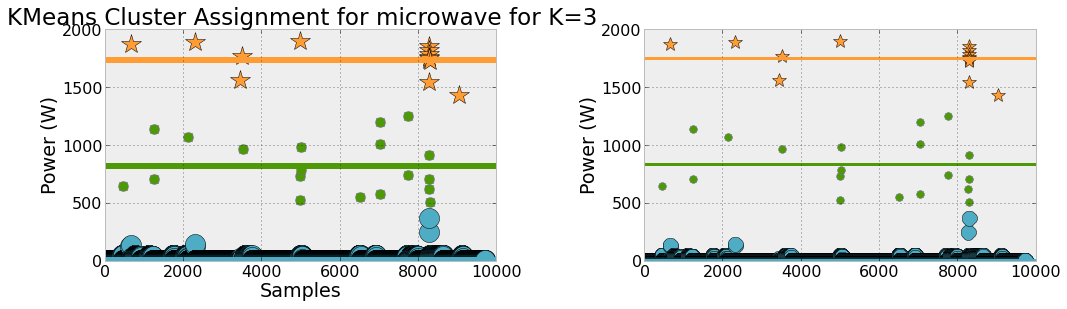
\includegraphics[width=0.7\textwidth]{REDD_House2_Analysis_files/REDD_House2_Analysis_fig_11.png}
\par
\end{center}
\begin{center}
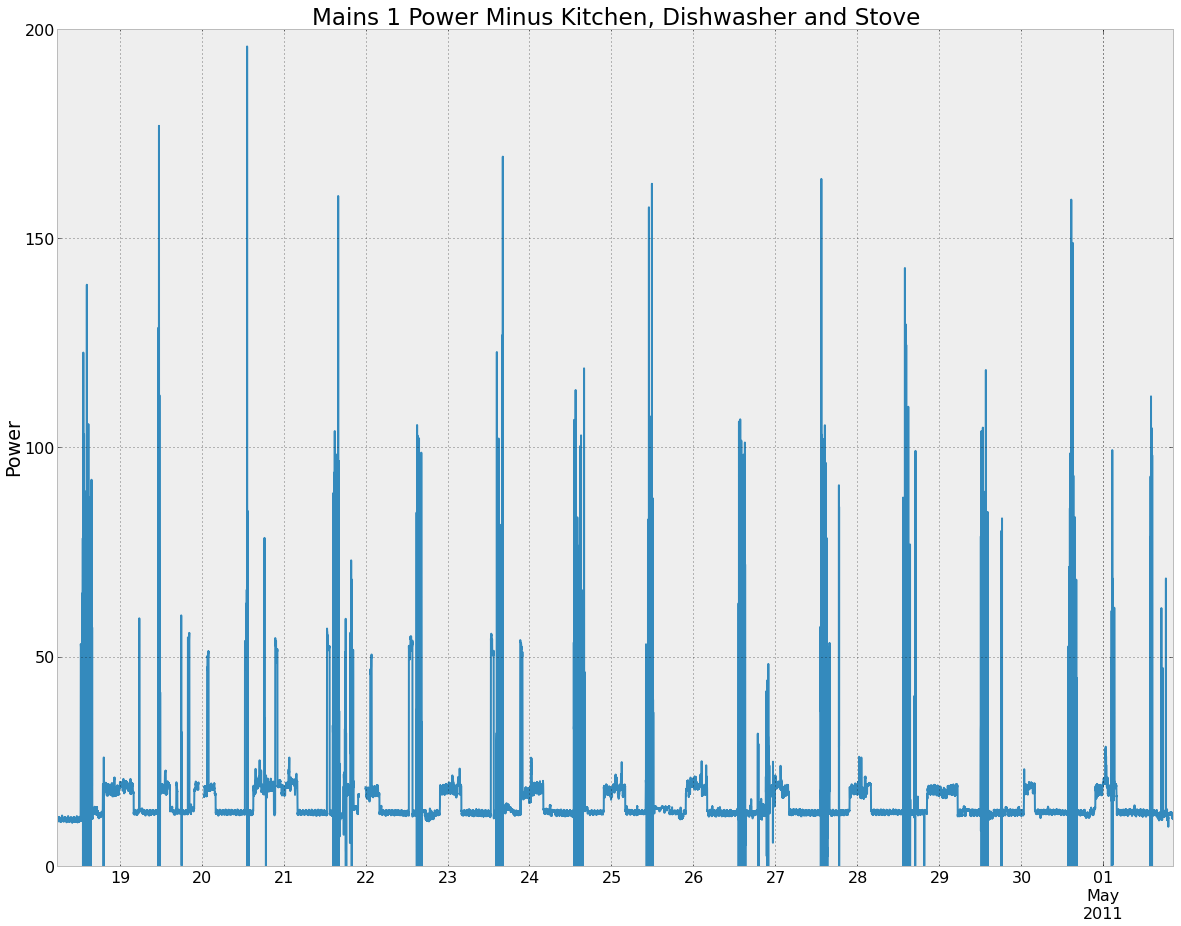
\includegraphics[width=0.7\textwidth]{REDD_House2_Analysis_files/REDD_House2_Analysis_fig_12.png}
\par
\end{center}
\end{codeoutput}
\end{codecell}
\begin{codecell}
\begin{codeinput}
\begin{lstlisting}
centroids
\end{lstlisting}
\end{codeinput}
\begin{codeoutput}
\begin{verbatim}
{'dishwasher': [0.1701359028503493, 1195.3713848039199, 260.53415359477123],
 'kitchen': [5.0765980080727378, 727.42865761689313],
 'kitchen_2': [1.4255969429011941, 1036.0540697674414, 204.70668553806448],
 'light': [9.4712692617067837, 156.30873674287119, 96.843738224826836],
 'microwave': [9.7741967140592507, 1740.2291666666672, 822.51469298245615],
 'refrigerator': [161.83612766450091, 7.4547324466263163, 423.53895502645537],
 'stove': [0.60312354161529014, 373.85056818181823]}
\end{verbatim}
\end{codeoutput}
\end{codecell}
Sorting centroids and also making the datatype integer

\begin{codecell}
\begin{codeinput}
\begin{lstlisting}
for appliance in centroids:
    centroids[appliance]=list(np.array(centroids[appliance]).astype(int))
    centroids[appliance].sort()
centroids
\end{lstlisting}
\end{codeinput}
\begin{codeoutput}
\begin{verbatim}
{'dishwasher': [0, 260, 1195],
 'kitchen': [5, 727],
 'kitchen_2': [1, 204, 1036],
 'light': [9, 96, 156],
 'microwave': [9, 822, 1740],
 'refrigerator': [7, 161, 423],
 'stove': [0, 373]}
\end{verbatim}
\end{codeoutput}
\end{codecell}
\subparagraph{Calibration}
No need for calibrating state 1 of each appliance since their power is
close to 0.

Finding events of transition from state 1 to 2 in Mains and in Appliance
and comparing them with cluster centroids assigned. Only if there are
greater than 10 number of transitions do we even consider the
calibration.

\begin{codecell}
\begin{codeinput}
\begin{lstlisting}

calib_centroids=deepcopy(centroids)
\end{lstlisting}
\end{codeinput}
\end{codecell}
\begin{codecell}
\begin{codeinput}
\begin{lstlisting}
for appliance in labels_appliance:
    l=labels_appliance[appliance]
    #print "%s has %d states" %(appliance,max(l)+1)
    
    #Finding factors for 2,..K th state
    #Note here indexing starts from 0 and not 1
    for k in range(1,max(l)+1):
        #Finding idx of where appliance is in state k-1 and next state is k
        idx=[]
        for i in range(len(l)-1):
            if l[i]==k-1 and l[i+1]==k:
                idx.append(i)
                
                diff_appliance=np.diff(df_appliances_train[appliance].values)
                diff_mains_1=np.diff(df_mains_train.Mains_1_Power.values)
                diff_mains_2=np.diff(df_mains_train.Mains_2_Power.values)
                
    
                if appliance in appliances_mains[0]:
                    x=diff_mains_1[idx]/diff_appliance[idx]
                    x=x[x<2]
                    x=x[x>0]
        
        
                else:
                    x=diff_mains_2[idx]/diff_appliance[idx]
                    x=x[x<2]
                    x=x[x>0]
        #print x,np.std(x)
        if (np.average(x)<0.9 or np.average(x)>1.1) and len(x)>10: 
            calib_centroids[appliance][k]=centroids[appliance][k]*np.average(x)
              
            print "Average for %s in %dth state is %f and number of transitions was %d" %(appliance,k+1,np.average(x),len(idx))

\end{lstlisting}
\end{codeinput}
\begin{codeoutput}
\begin{verbatim}
Average for light in 2th state is 1.178171 and number of transitions was 16
Average for refrigerator in 2th state is 1.330662 and number of transitions was 178
\end{verbatim}
\begin{verbatim}

\end{verbatim}
\end{codeoutput}
\end{codecell}
After calibration the power in different states is given below.

\begin{codecell}
\begin{codeinput}
\begin{lstlisting}
for appliance in calib_centroids:
    calib_centroids[appliance]=list(np.array(calib_centroids[appliance]).astype(int))
    
pprint.pprint(calib_centroids)       
\end{lstlisting}
\end{codeinput}
\begin{codeoutput}
\begin{verbatim}
{'dishwasher': [0, 260, 1195],
 'kitchen': [5, 727],
 'kitchen_2': [1, 204, 1036],
 'light': [9, 113, 156],
 'microwave': [9, 822, 1740],
 'refrigerator': [7, 214, 423],
 'stove': [0, 373]}
\end{verbatim}
\end{codeoutput}
\end{codecell}
\subparagraph{CO based NIALM}
\begin{codecell}
\begin{codeinput}
\begin{lstlisting}
def find_nearest_index(array,value):
    idx = (np.abs(array-value)).argmin()
    return idx
def find_labels(appliance_power_consumption_list, observed_power):
    labels=np.zeros(len(observed_power))
    appliance_power_consumption_array=np.array(appliance_power_consumption_list)
    for i in range(len(observed_power)):
        labels[i]=find_nearest_index(appliance_power_consumption_array,observed_power[i])
    return labels
\end{lstlisting}
\end{codeinput}
\end{codecell}
Finding true labels of appliances on the test set

\begin{codecell}
\begin{codeinput}
\begin{lstlisting}
true_labels={}
for appliance in centroids:
    true_labels[appliance]=find_labels(centroids[appliance], df_appliances_test[appliance])
    
\end{lstlisting}
\end{codeinput}
\end{codecell}
\begin{codecell}
\begin{codeinput}
\begin{lstlisting}
def print_confusion_matrix(appliance,num_states,true_label,observed_label):
    correct_predicted=0
    conf_arr=[]
    for i in range(num_states):
        counts=[]
        for j in range(num_states):        
            idx=np.where(true_label==i)[0]
            counts.append(len(np.where(observed_label[idx]==j)[0]))
        correct_predicted+=counts[i]
        conf_arr.append(counts)
    
    norm_conf = []
    for i in conf_arr:
        a = 0
        tmp_arr = []
        a = sum(i, 0)
        for j in i:
            tmp_arr.append(float(j)/float(a))
        norm_conf.append(tmp_arr)

    fig = plt.figure()
    plt.clf()
    ax = fig.add_subplot(111)
    ax.set_aspect(1)
    res = ax.imshow(np.array(norm_conf), cmap=plt.cm.jet, 
                interpolation='nearest')

    width = len(conf_arr)
    height = len(conf_arr[0])

    for x in xrange(width):
        for y in xrange(height):
            ax.annotate(str(conf_arr[x][y]), xy=(y, x), 
                    horizontalalignment='center',
                    verticalalignment='center')

    cb = fig.colorbar(res)
    alphabet = ['State 1','State 2','State 3']
    plt.title('Confusion Matrix for '+appliance)
    plt.xticks(range(width), alphabet[:width])
    plt.yticks(range(height), alphabet[:height])
    plt.show()
    return correct_predicted*1.0/len(true_label)  
\end{lstlisting}
\end{codeinput}
\end{codecell}
\subsubsection{Without Calibration}
\paragraph{Without load division}
\begin{codecell}
\begin{codeinput}
\begin{lstlisting}
def find_nearest(array,value):
    idx = (np.abs(array-value)).argmin()
    diff=array[idx]-value
    return [idx,-diff]
\end{lstlisting}
\end{codeinput}
\end{codecell}
\begin{codecell}
\begin{codeinput}
\begin{lstlisting}
states_combination=list(itertools.product(centroids['kitchen'],centroids['stove'],\
centroids['kitchen_2'],centroids['dishwasher'],centroids['refrigerator'],centroids['light'],\
centroids['microwave']))
sum_combination=np.array(np.zeros(len(states_combination)))
for i in range(0,len(states_combination)):
    sum_combination[i]=sum(states_combination[i])


\end{lstlisting}
\end{codeinput}
\end{codecell}
\begin{codecell}
\begin{codeinput}
\begin{lstlisting}
length_sequence=len(df_mains_test.Mains_1_Power.values)
states=np.zeros(length_sequence)
residual_power=np.zeros(length_sequence)
t0=time.time()
for i in range(length_sequence):
    [states[i],residual_power[i]]=find_nearest(sum_combination,df_mains_test.Mains_2_Power.values[i]+df_mains_test.Mains_1_Power.values[i])
t1=time.time()
print "Time taken for CO Mains 2 :",t1-t0
\end{lstlisting}
\end{codeinput}
\begin{codeoutput}
\begin{verbatim}
Time taken for CO Mains 2 : 0.30699300766
\end{verbatim}
\end{codeoutput}
\end{codecell}
\begin{codecell}
\begin{codeinput}
\begin{lstlisting}
def decode_CO(length_sequence,centroids,appliance_list,states,residual_power):
    
    co_states={}
    co_power={}
    total_num_combinations=1
    for appliance in appliance_list:
        total_num_combinations*=len(centroids[appliance])
   

    for appliance in appliance_list:
        co_states[appliance]=np.zeros(length_sequence,dtype=np.int)
        co_power[appliance]=np.zeros(length_sequence)
    
    for i in range(length_sequence):
        factor=total_num_combinations
        for appliance in appliance_list:
            #assuming integer division (will cause errors in Python 3x)
            factor=factor/len(centroids[appliance])
            
            temp=int(states[i])/factor
            co_states[appliance][i]=temp%len(centroids[appliance])
            co_power[appliance][i]=centroids[appliance][co_states[appliance][i]]
            
    return [co_states,co_power]
    
\end{lstlisting}
\end{codeinput}
\end{codecell}
\begin{codecell}
\begin{codeinput}
\begin{lstlisting}
appliance_list=['kitchen','stove','kitchen_2','dishwasher','refrigerator','light','microwave']
\end{lstlisting}
\end{codeinput}
\end{codecell}
\begin{codecell}
\begin{codeinput}
\begin{lstlisting}
[case_1_states,case_1_power]=decode_CO(length_sequence,centroids,appliance_list,states,residual_power)
\end{lstlisting}
\end{codeinput}
\end{codecell}
Printing confusion matrices

\begin{codecell}
\begin{codeinput}
\begin{lstlisting}
for appliance in appliance_list:
    print_confusion_matrix(appliance,len(centroids[appliance]),true_labels[appliance],case_1_states[appliance])
\end{lstlisting}
\end{codeinput}
\begin{codeoutput}
\begin{center}
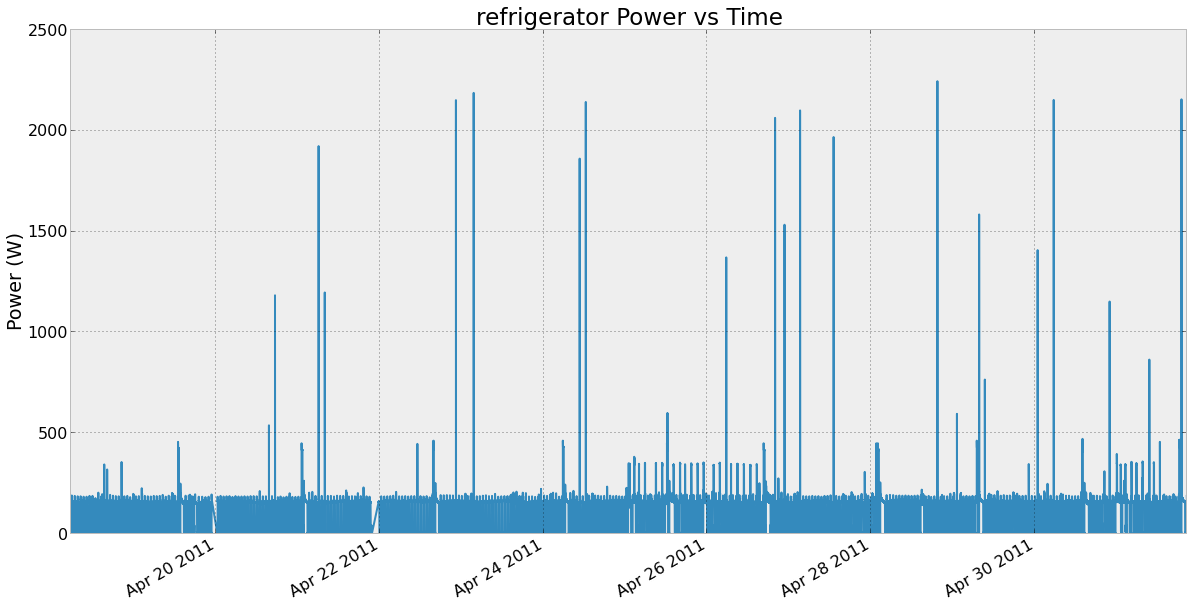
\includegraphics[width=0.7\textwidth]{REDD_House2_Analysis_files/REDD_House2_Analysis_fig_13.png}
\par
\end{center}
\begin{center}
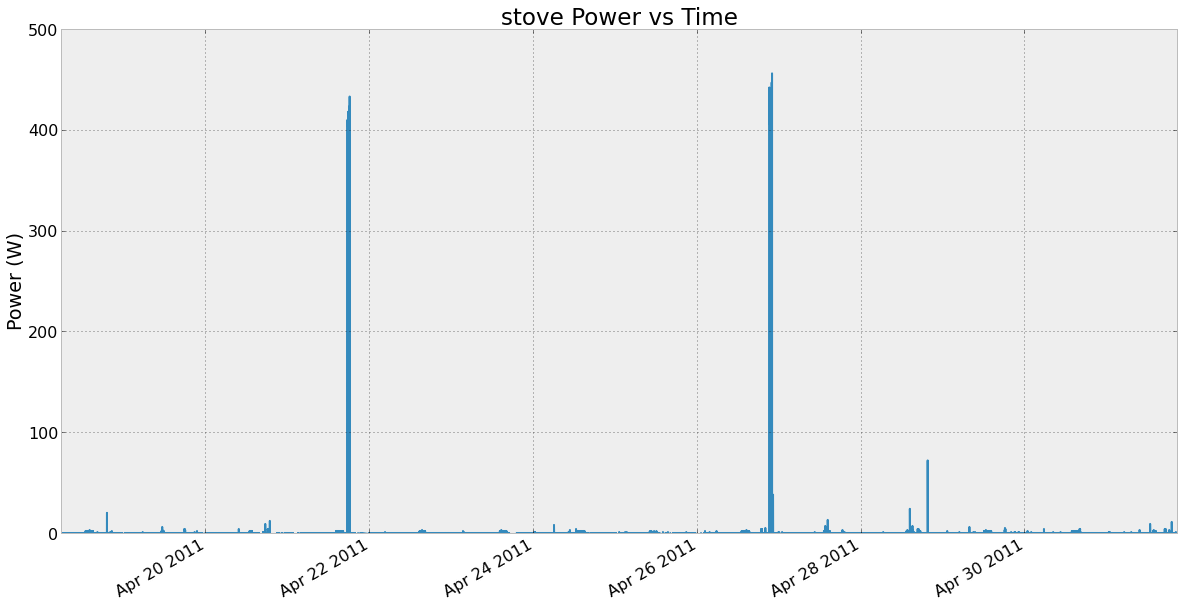
\includegraphics[width=0.7\textwidth]{REDD_House2_Analysis_files/REDD_House2_Analysis_fig_14.png}
\par
\end{center}
\begin{center}
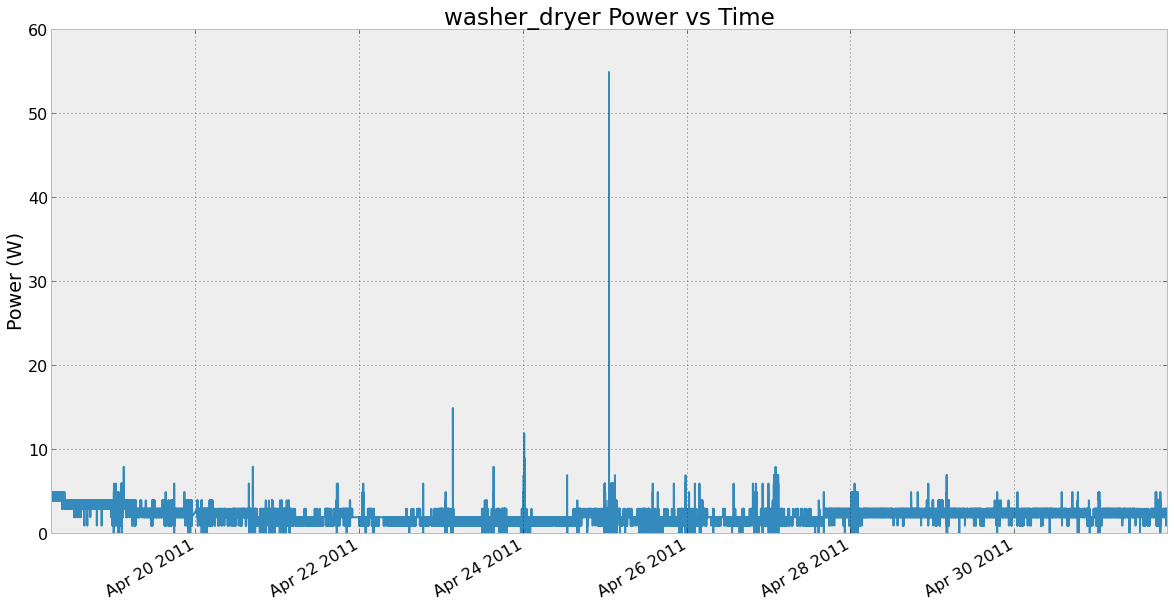
\includegraphics[width=0.7\textwidth]{REDD_House2_Analysis_files/REDD_House2_Analysis_fig_15.png}
\par
\end{center}
\begin{center}
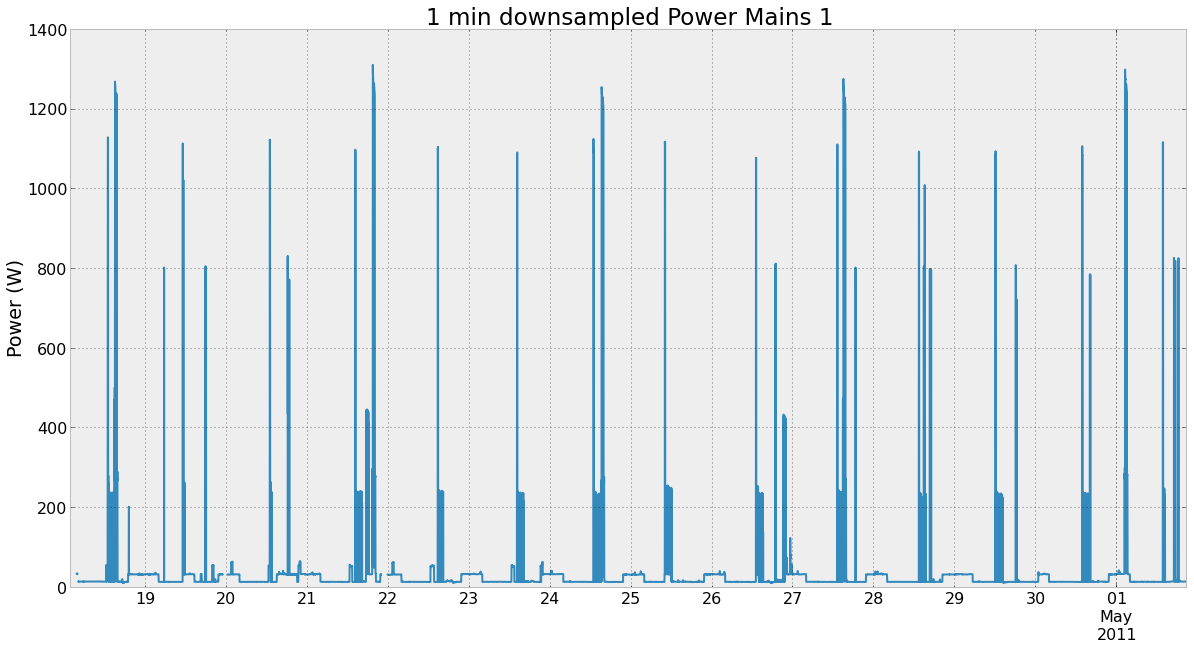
\includegraphics[width=0.7\textwidth]{REDD_House2_Analysis_files/REDD_House2_Analysis_fig_16.png}
\par
\end{center}
\begin{center}
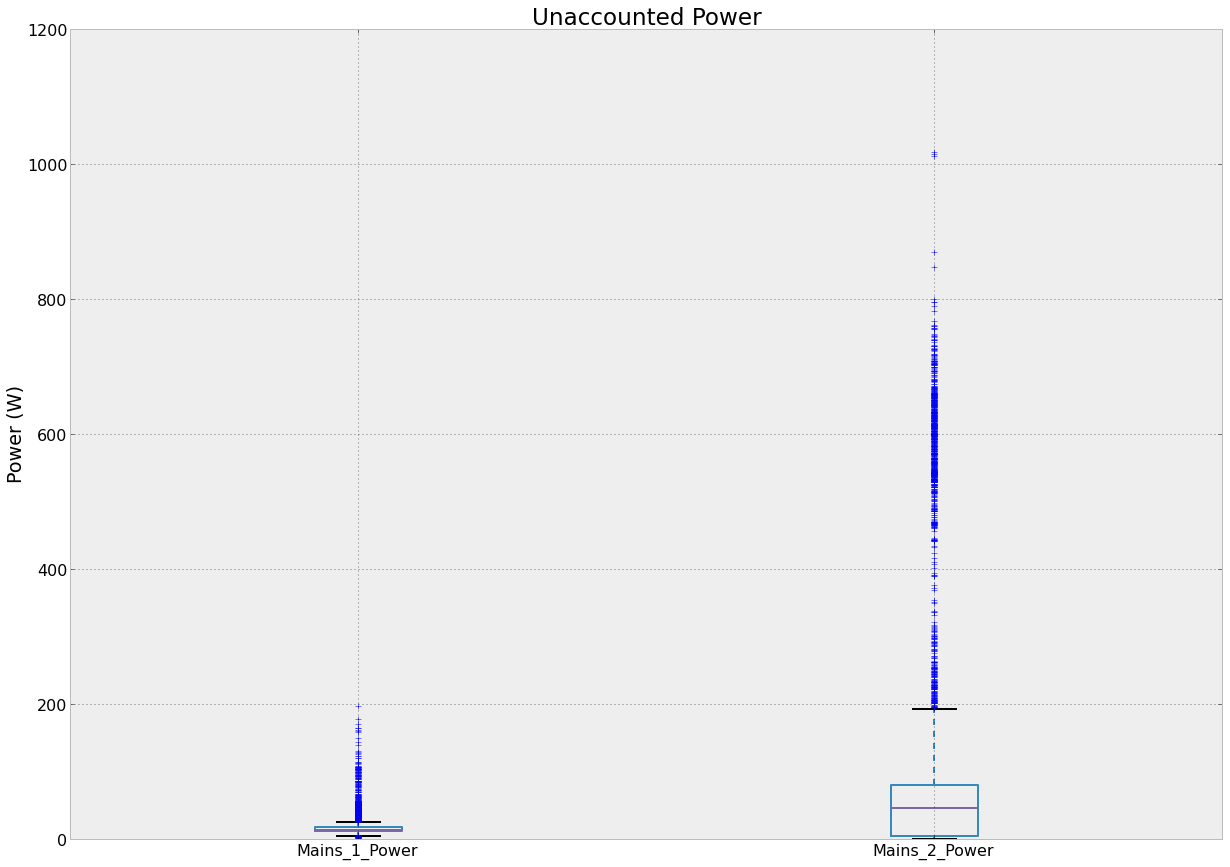
\includegraphics[width=0.7\textwidth]{REDD_House2_Analysis_files/REDD_House2_Analysis_fig_17.png}
\par
\end{center}
\begin{center}
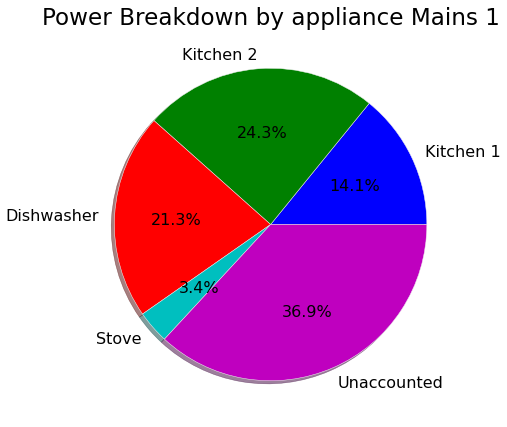
\includegraphics[width=0.7\textwidth]{REDD_House2_Analysis_files/REDD_House2_Analysis_fig_18.png}
\par
\end{center}
\begin{center}
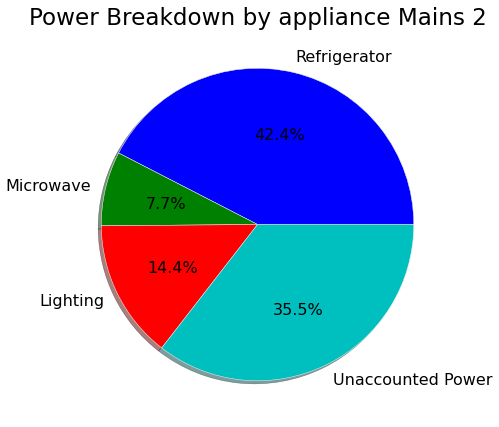
\includegraphics[width=0.7\textwidth]{REDD_House2_Analysis_files/REDD_House2_Analysis_fig_19.png}
\par
\end{center}
\end{codeoutput}
\end{codecell}
\begin{codecell}
\begin{codeinput}
\begin{lstlisting}
MNE=[]
RE=[]
\end{lstlisting}
\end{codeinput}
\end{codecell}
\begin{codecell}
\begin{codeinput}
\begin{lstlisting}
numerator={}
denominator={}
mne={}
re={}
for appliance in case_1_states:
    numerator[appliance]=np.sum(np.abs(case_1_power[appliance]-df_appliances_test[appliance].values))
    denominator[appliance]=np.sum(df_appliances_test[appliance].values)
    mne[appliance]=numerator[appliance]*1.0/denominator[appliance]
    re[appliance]=np.std(case_1_power[appliance]-df_appliances_test[appliance].values)
    
MNE.append(deepcopy(mne))
RE.append(deepcopy(re))

\end{lstlisting}
\end{codeinput}
\end{codecell}
\paragraph{With load division}
Mains 1

\begin{codecell}
\begin{codeinput}
\begin{lstlisting}
states_combination=list(itertools.product(centroids['kitchen'],centroids['stove'],\
centroids['kitchen_2'],centroids['dishwasher']))
sum_combination=np.array(np.zeros(len(states_combination)))
for i in range(0,len(states_combination)):
    sum_combination[i]=sum(states_combination[i])
    
length_sequence=len(df_mains_test.Mains_1_Power.values)
states=np.zeros(length_sequence)
residual_power=np.zeros(length_sequence)
t0=time.time()
for i in range(length_sequence):
    [states[i],residual_power[i]]=find_nearest(sum_combination,df_mains_test.Mains_1_Power.values[i])
t1=time.time()
print "Time taken for CO Mains :",t1-t0

appliance_list=['kitchen','stove','kitchen_2','dishwasher']


[case_2_mains_1_states,case_2_mains_1_power]=decode_CO(length_sequence,centroids,appliance_list,states,residual_power)
\end{lstlisting}
\end{codeinput}
\begin{codeoutput}
\begin{verbatim}
Time taken for CO Mains : 0.1943359375
\end{verbatim}
\end{codeoutput}
\end{codecell}
\begin{codecell}
\begin{codeinput}
\begin{lstlisting}
for appliance in appliance_list:
    figure()
    plt.subplot(2,1,1)
    plt.title(appliance)
    plt.plot(df_appliances_test[appliance].values)
    plt.subplot(2,1,2)
    plt.plot(case_2_mains_1_power[appliance])
             
    print_confusion_matrix(appliance,len(centroids[appliance]),true_labels[appliance],case_2_mains_1_states[appliance])
\end{lstlisting}
\end{codeinput}
\begin{codeoutput}
\begin{center}
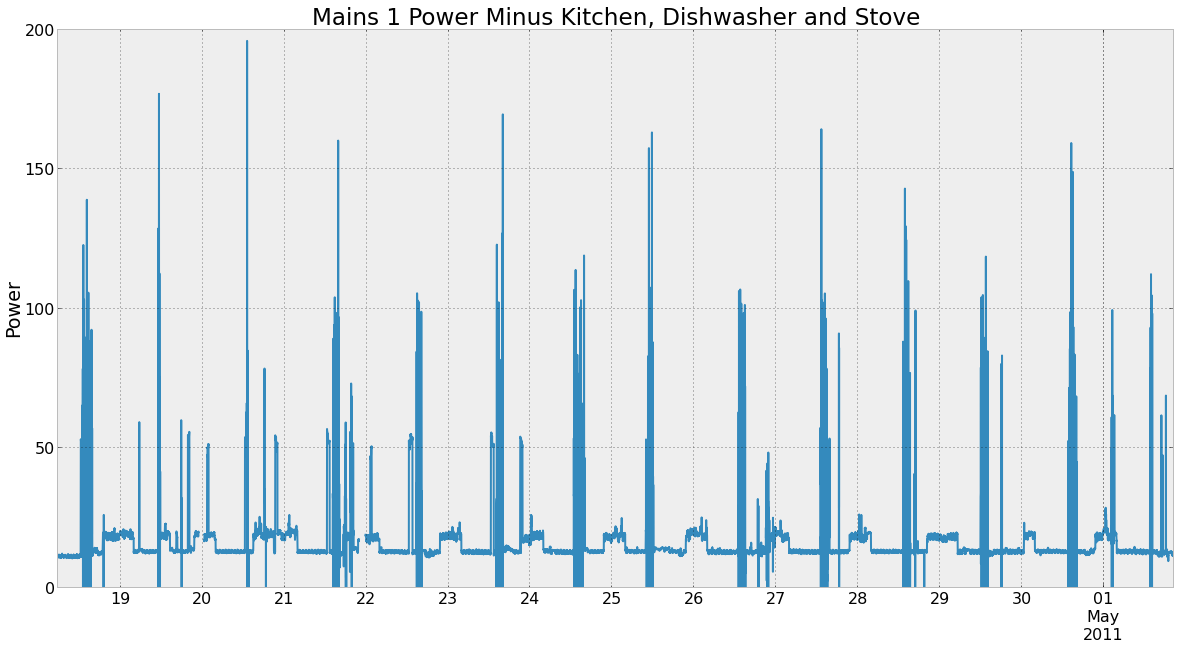
\includegraphics[width=0.7\textwidth]{REDD_House2_Analysis_files/REDD_House2_Analysis_fig_20.png}
\par
\end{center}
\begin{center}
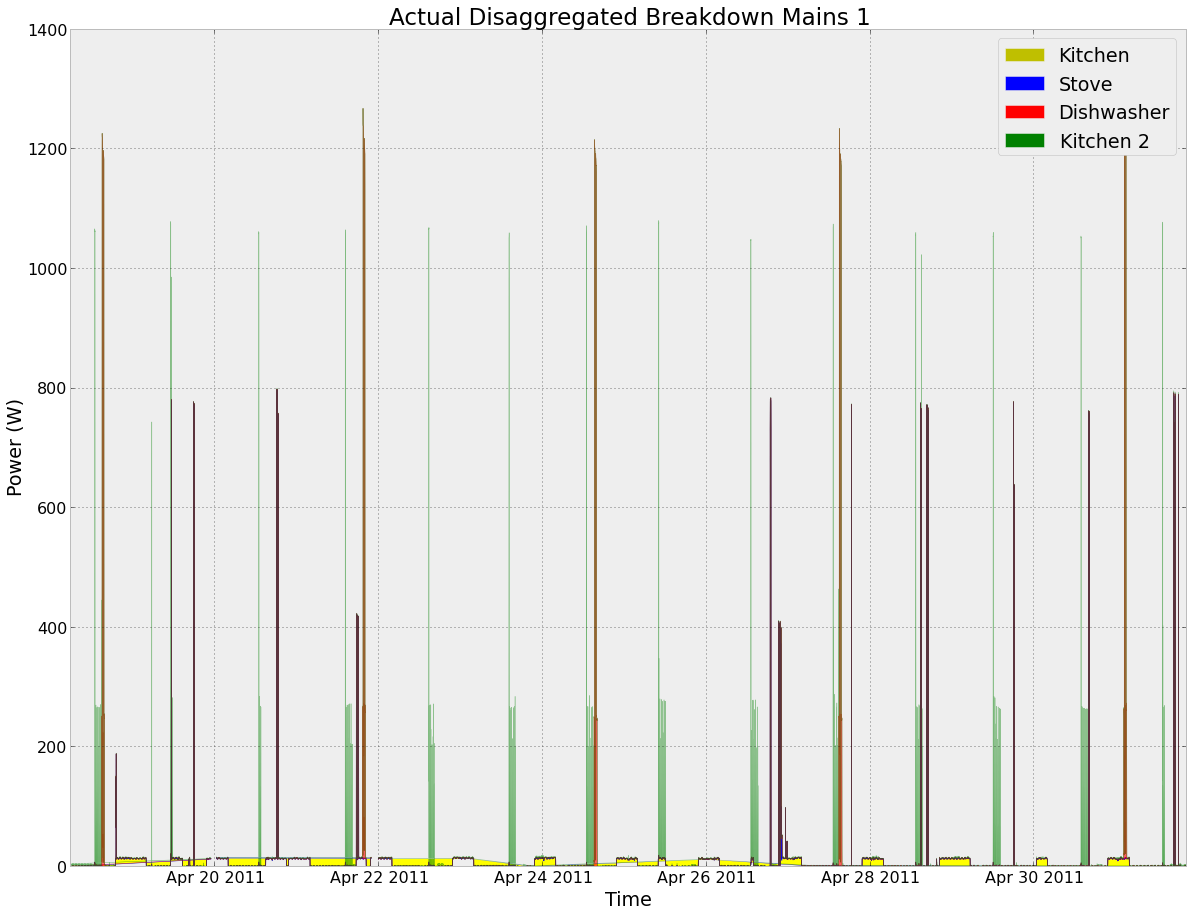
\includegraphics[width=0.7\textwidth]{REDD_House2_Analysis_files/REDD_House2_Analysis_fig_21.png}
\par
\end{center}
\begin{center}
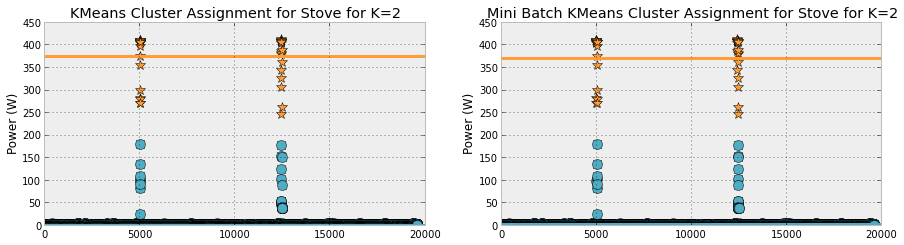
\includegraphics[width=0.7\textwidth]{REDD_House2_Analysis_files/REDD_House2_Analysis_fig_22.png}
\par
\end{center}
\begin{center}
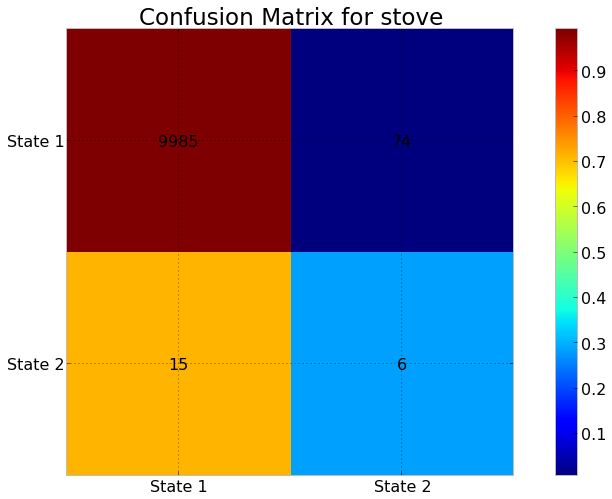
\includegraphics[width=0.7\textwidth]{REDD_House2_Analysis_files/REDD_House2_Analysis_fig_23.png}
\par
\end{center}
\begin{center}
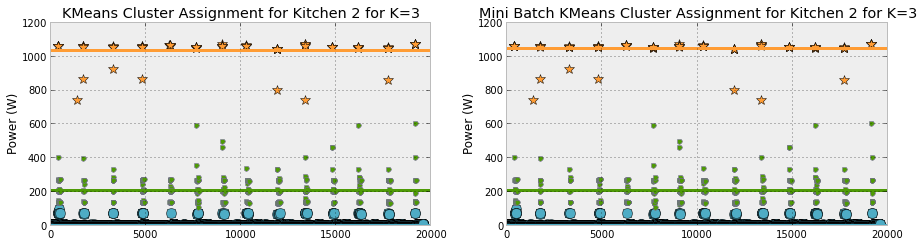
\includegraphics[width=0.7\textwidth]{REDD_House2_Analysis_files/REDD_House2_Analysis_fig_24.png}
\par
\end{center}
\begin{center}
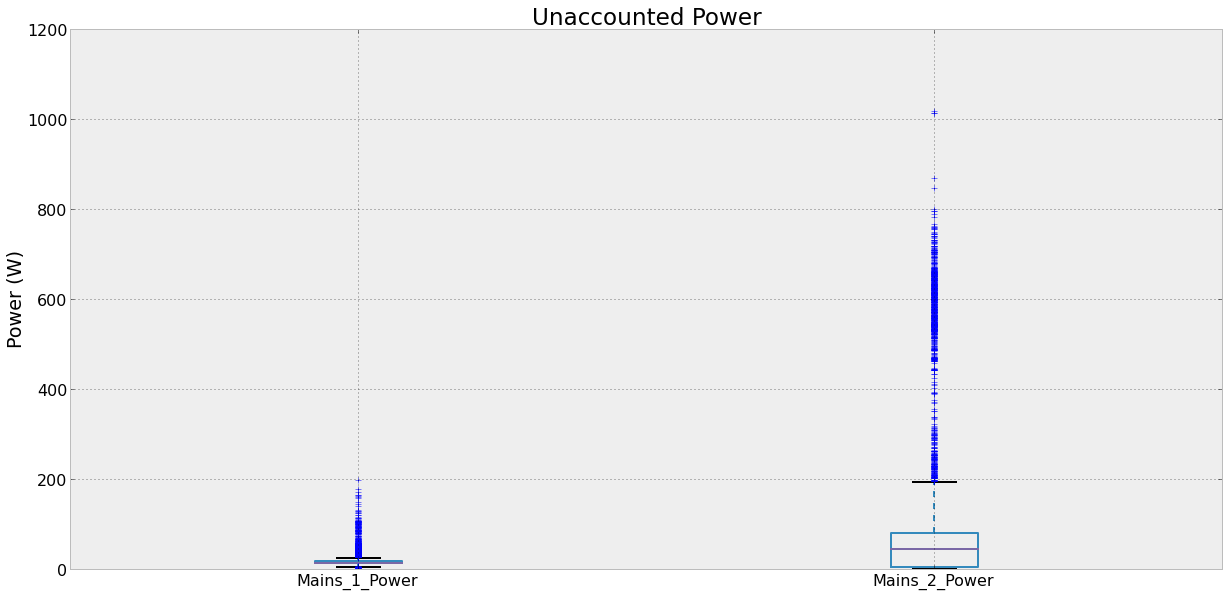
\includegraphics[width=0.7\textwidth]{REDD_House2_Analysis_files/REDD_House2_Analysis_fig_25.png}
\par
\end{center}
\begin{center}
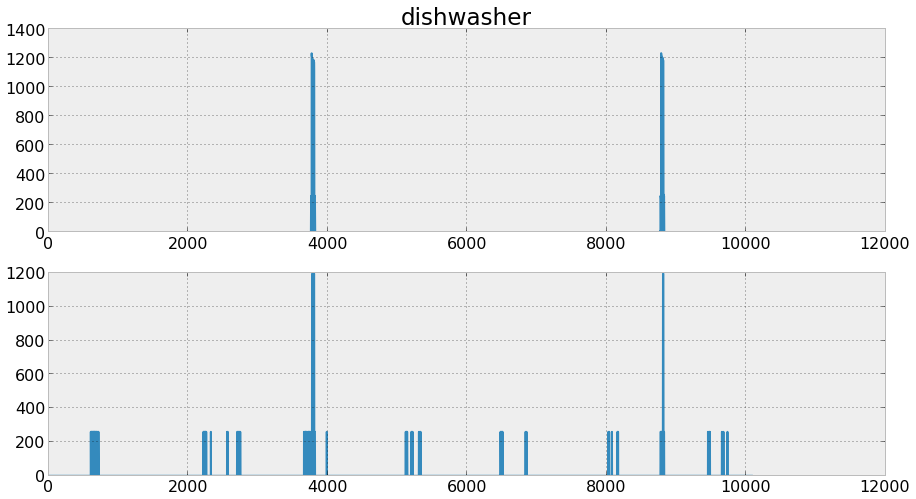
\includegraphics[width=0.7\textwidth]{REDD_House2_Analysis_files/REDD_House2_Analysis_fig_26.png}
\par
\end{center}
\begin{center}
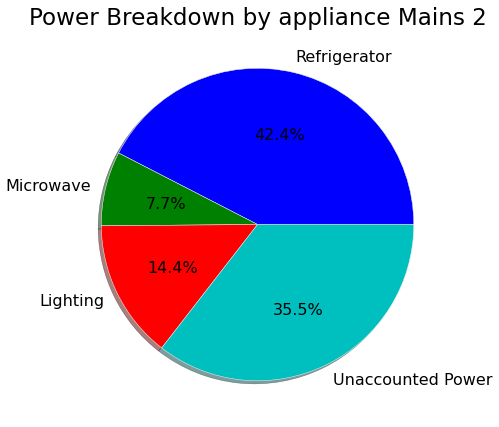
\includegraphics[width=0.7\textwidth]{REDD_House2_Analysis_files/REDD_House2_Analysis_fig_27.png}
\par
\end{center}
\end{codeoutput}
\end{codecell}
\begin{codecell}
\begin{codeinput}
\begin{lstlisting}
numerator={}
denominator={}
mne={}
re={}
for appliance in appliance_list:
    numerator[appliance]=np.sum(np.abs(case_2_mains_1_power[appliance]-df_appliances_test[appliance].values))
    denominator[appliance]=np.sum(df_appliances_test[appliance].values)
    mne[appliance]=numerator[appliance]*1.0/denominator[appliance]
    re[appliance]=np.std(case_2_mains_1_power[appliance]-df_appliances_test[appliance].values)

\end{lstlisting}
\end{codeinput}
\end{codecell}
Mains 2

\begin{codecell}
\begin{codeinput}
\begin{lstlisting}
states_combination=list(itertools.product(centroids['refrigerator'],centroids['light'],\
centroids['microwave']))
sum_combination=np.array(np.zeros(len(states_combination)))
for i in range(0,len(states_combination)):
    sum_combination[i]=sum(states_combination[i])
\end{lstlisting}
\end{codeinput}
\end{codecell}
\begin{codecell}
\begin{codeinput}
\begin{lstlisting}
length_sequence=len(df_mains_test.Mains_2_Power.values)
states=np.zeros(length_sequence)
residual_power=np.zeros(length_sequence)
t0=time.time()
for i in range(length_sequence):
    [states[i],residual_power[i]]=find_nearest(sum_combination,df_mains_test.Mains_2_Power.values[i])
t1=time.time()
print "Time taken for CO Mains :",t1-t0
print residual_power
\end{lstlisting}
\end{codeinput}
\begin{codeoutput}
\begin{verbatim}
Time taken for CO Mains : 0.194933891296
[-14.93716667 -15.91083333 -16.59033333 ...,  25.695       25.25240741
  25.46854545]
\end{verbatim}
\end{codeoutput}
\end{codecell}
\begin{codecell}
\begin{codeinput}
\begin{lstlisting}
appliance_list=['refrigerator','light','microwave']
\end{lstlisting}
\end{codeinput}
\end{codecell}
\begin{codecell}
\begin{codeinput}
\begin{lstlisting}
[case_2_mains_2_states,case_2_mains_2_power]=decode_CO(length_sequence,centroids,appliance_list,states,residual_power)
\end{lstlisting}
\end{codeinput}
\end{codecell}
\begin{codecell}
\begin{codeinput}
\begin{lstlisting}
case_2_mains_2_states
\end{lstlisting}
\end{codeinput}
\begin{codeoutput}
\begin{verbatim}
{'light': array([1, 1, 1, ..., 1, 1, 1]),
 'microwave': array([0, 0, 0, ..., 0, 0, 0]),
 'refrigerator': array([1, 1, 1, ..., 0, 0, 0])}
\end{verbatim}
\end{codeoutput}
\end{codecell}
\begin{codecell}
\begin{codeinput}
\begin{lstlisting}
for appliance in appliance_list:
    figure()
    plt.subplot(2,1,1)
    plt.title(appliance)
    plt.plot(df_appliances_test[appliance].values)
    plt.subplot(2,1,2)
    plt.plot(case_2_mains_2_power[appliance])
             
    print_confusion_matrix(appliance,len(centroids[appliance]),true_labels[appliance],case_2_mains_2_states[appliance])
\end{lstlisting}
\end{codeinput}
\begin{codeoutput}
\begin{center}
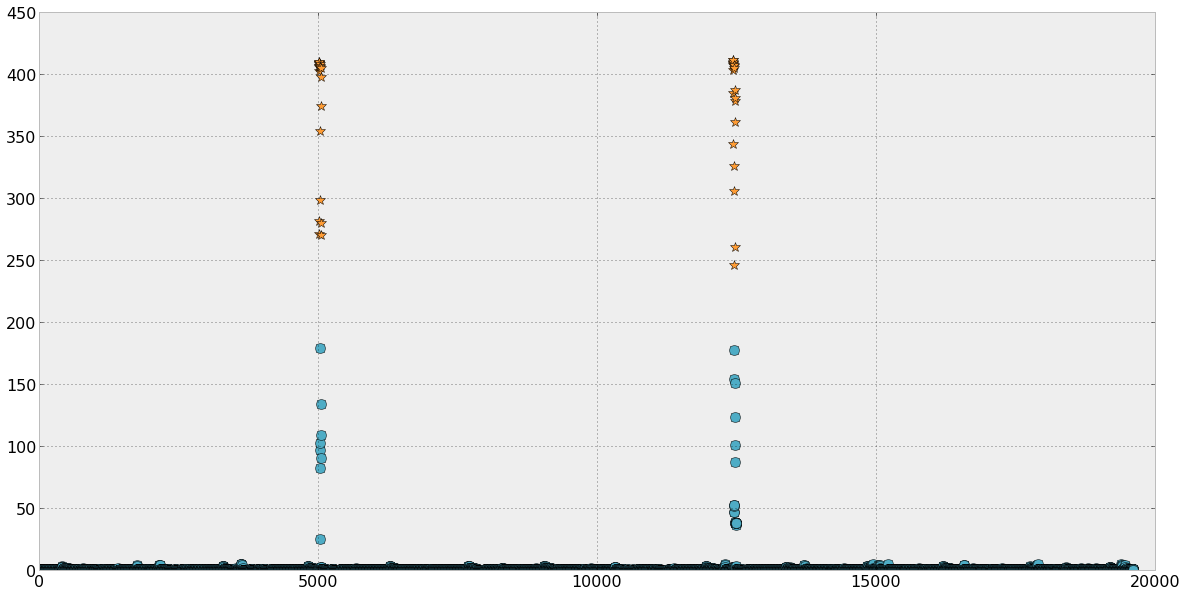
\includegraphics[width=0.7\textwidth]{REDD_House2_Analysis_files/REDD_House2_Analysis_fig_28.png}
\par
\end{center}
\begin{center}
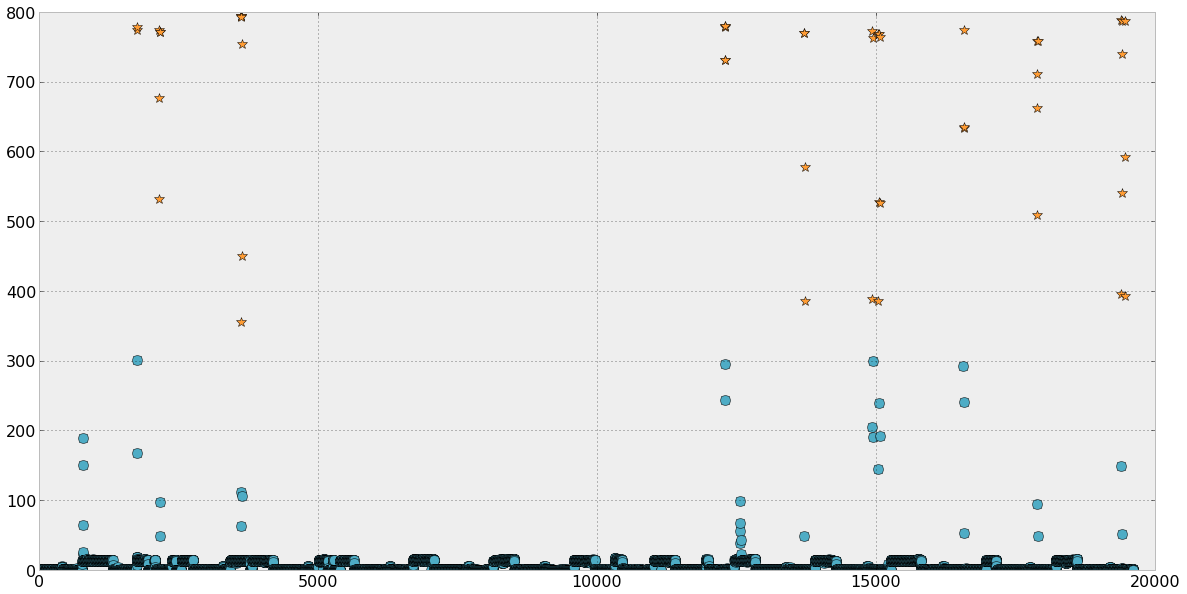
\includegraphics[width=0.7\textwidth]{REDD_House2_Analysis_files/REDD_House2_Analysis_fig_29.png}
\par
\end{center}
\begin{center}
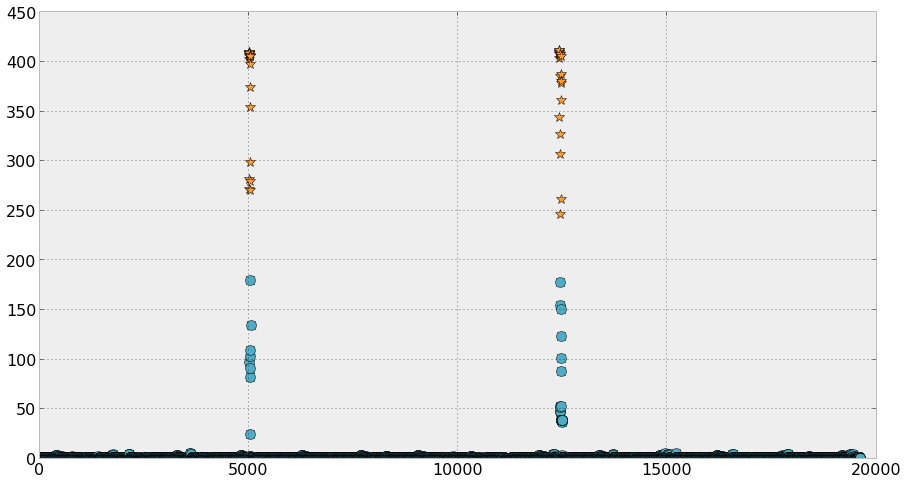
\includegraphics[width=0.7\textwidth]{REDD_House2_Analysis_files/REDD_House2_Analysis_fig_30.png}
\par
\end{center}
\begin{center}
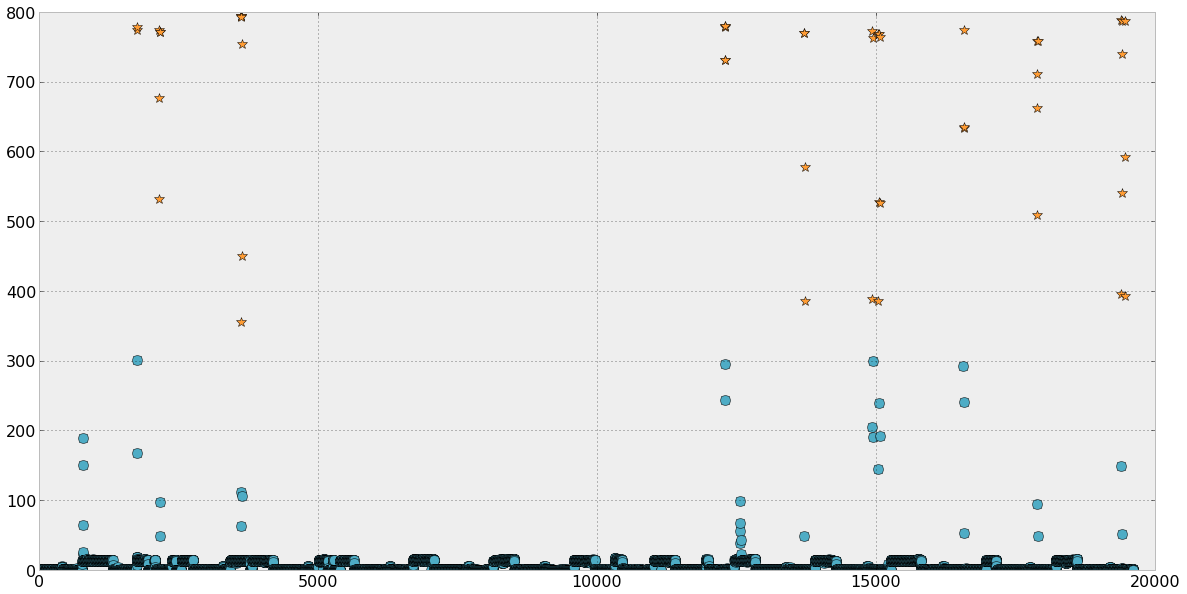
\includegraphics[width=0.7\textwidth]{REDD_House2_Analysis_files/REDD_House2_Analysis_fig_31.png}
\par
\end{center}
\begin{center}
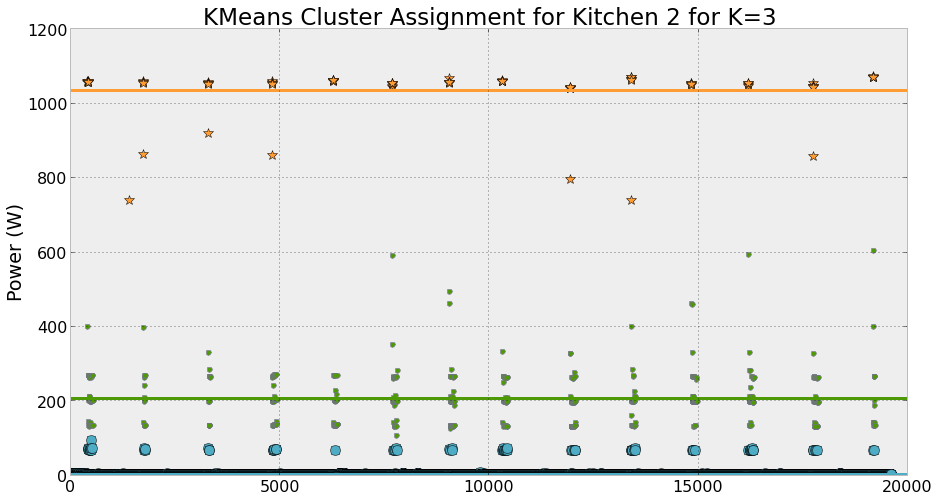
\includegraphics[width=0.7\textwidth]{REDD_House2_Analysis_files/REDD_House2_Analysis_fig_32.png}
\par
\end{center}
\begin{center}
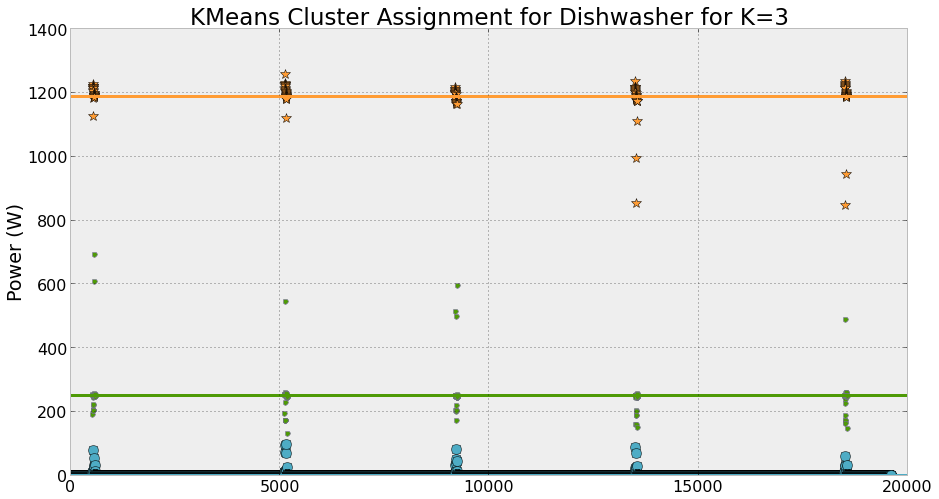
\includegraphics[width=0.7\textwidth]{REDD_House2_Analysis_files/REDD_House2_Analysis_fig_33.png}
\par
\end{center}
\end{codeoutput}
\end{codecell}
\begin{codecell}
\begin{codeinput}
\begin{lstlisting}
numerator={}
denominator={}
for appliance in appliance_list:
    numerator[appliance]=np.sum(np.abs(case_2_mains_2_power[appliance]-df_appliances_test[appliance].values))
    denominator[appliance]=np.sum(df_appliances_test[appliance].values)
    mne[appliance]=numerator[appliance]*1.0/denominator[appliance]
    re[appliance]=np.std(case_2_mains_2_power[appliance]-df_appliances_test[appliance].values)

    
MNE.append(deepcopy(mne))
RE.append(deepcopy(re))

\end{lstlisting}
\end{codeinput}
\end{codecell}
\subsubsection{With Calibration}
\paragraph{Without Load Division}
\begin{codecell}
\begin{codeinput}
\begin{lstlisting}
states_combination=list(itertools.product(calib_centroids['kitchen'],calib_centroids['stove'],calib_centroids['kitchen_2'],calib_centroids['dishwasher'],calib_centroids['refrigerator'],calib_centroids['light'],calib_centroids['microwave']))
sum_combination=np.array(np.zeros(len(states_combination)))
for i in range(0,len(states_combination)):
    sum_combination[i]=sum(states_combination[i])

\end{lstlisting}
\end{codeinput}
\end{codecell}
\begin{codecell}
\begin{codeinput}
\begin{lstlisting}
length_sequence=len(df_mains_test.Mains_1_Power.values)
states=np.zeros(length_sequence)
residual_power=np.zeros(length_sequence)
t0=time.time()
for i in range(length_sequence):
    [states[i],residual_power[i]]=find_nearest(sum_combination,df_mains_test.Mains_2_Power.values[i]+df_mains_test.Mains_1_Power.values[i])
t1=time.time()
print "Time taken for CO Mains 2 :",t1-t0
\end{lstlisting}
\end{codeinput}
\begin{codeoutput}
\begin{verbatim}
Time taken for CO Mains 2 : 0.301403045654
\end{verbatim}
\end{codeoutput}
\end{codecell}
\begin{codecell}
\begin{codeinput}
\begin{lstlisting}
appliance_list=['kitchen','stove','kitchen_2','dishwasher','refrigerator','light','microwave']
\end{lstlisting}
\end{codeinput}
\end{codecell}
\begin{codecell}
\begin{codeinput}
\begin{lstlisting}
[case_3_states,case_3_power]=decode_CO(length_sequence,centroids,appliance_list,states,residual_power)
\end{lstlisting}
\end{codeinput}
\end{codecell}
\begin{codecell}
\begin{codeinput}
\begin{lstlisting}
for appliance in appliance_list:
    print_confusion_matrix(appliance,len(calib_centroids[appliance]),true_labels[appliance],case_3_states[appliance])
\end{lstlisting}
\end{codeinput}
\begin{codeoutput}
\begin{center}
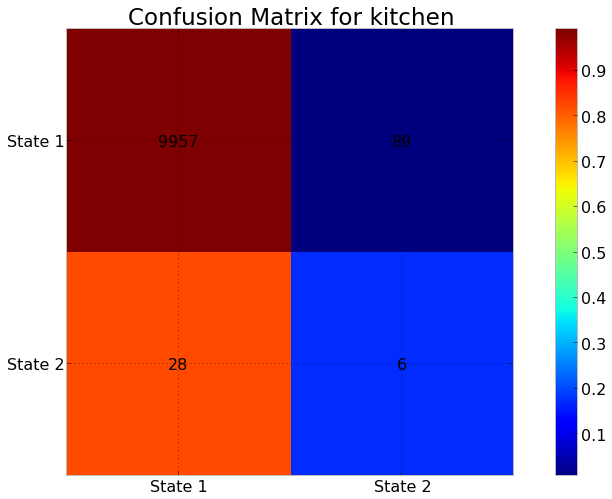
\includegraphics[width=0.7\textwidth]{REDD_House2_Analysis_files/REDD_House2_Analysis_fig_34.png}
\par
\end{center}
\begin{center}
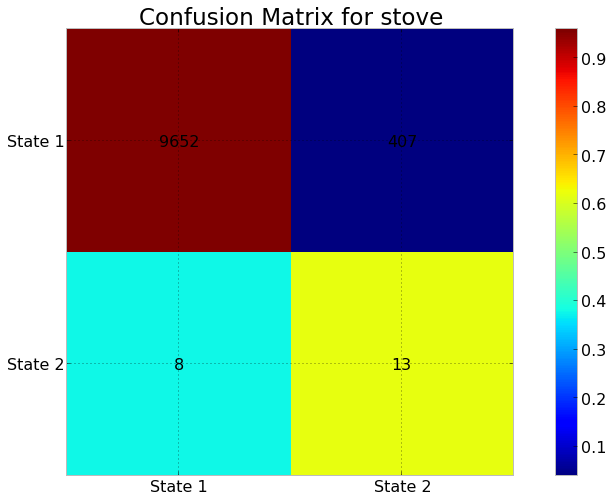
\includegraphics[width=0.7\textwidth]{REDD_House2_Analysis_files/REDD_House2_Analysis_fig_35.png}
\par
\end{center}
\begin{center}
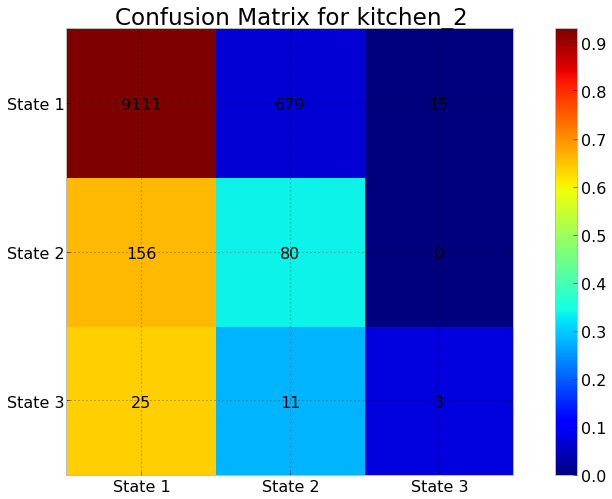
\includegraphics[width=0.7\textwidth]{REDD_House2_Analysis_files/REDD_House2_Analysis_fig_36.png}
\par
\end{center}
\begin{center}
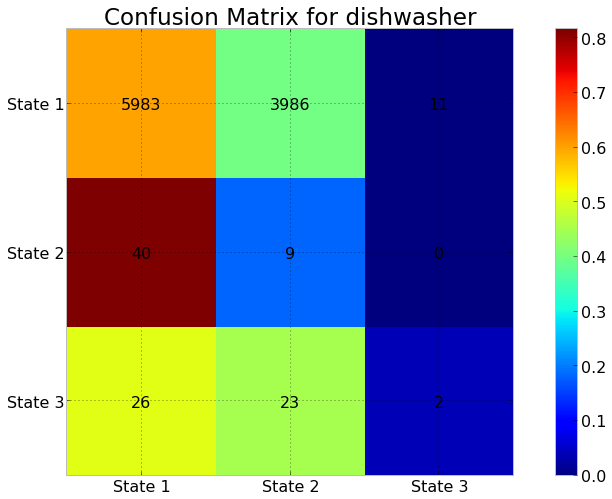
\includegraphics[width=0.7\textwidth]{REDD_House2_Analysis_files/REDD_House2_Analysis_fig_37.png}
\par
\end{center}
\begin{center}
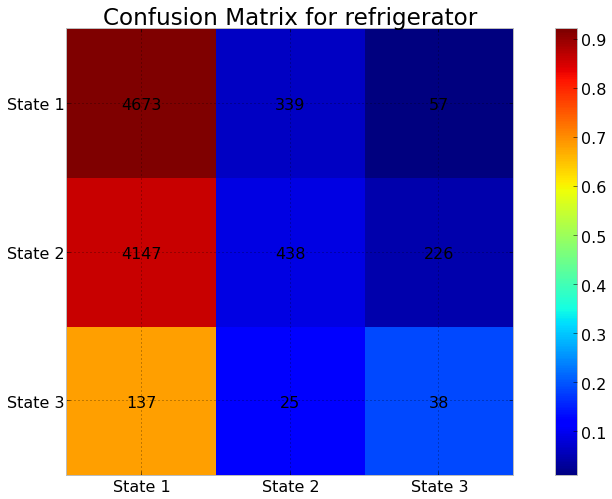
\includegraphics[width=0.7\textwidth]{REDD_House2_Analysis_files/REDD_House2_Analysis_fig_38.png}
\par
\end{center}
\begin{center}
\includegraphics[width=0.7\textwidth]{REDD_House2_Analysis_files/REDD_House2_Analysis_fig_39.png}
\par
\end{center}
\begin{center}
\includegraphics[width=0.7\textwidth]{REDD_House2_Analysis_files/REDD_House2_Analysis_fig_40.png}
\par
\end{center}
\end{codeoutput}
\end{codecell}
\begin{codecell}
\begin{codeinput}
\begin{lstlisting}
numerator={}
denominator={}
case=2
mne={}
re={}
for appliance in case_3_states:
    numerator[appliance]=np.sum(np.abs(case_3_power[appliance]-df_appliances_test[appliance].values))
    denominator[appliance]=np.sum(df_appliances_test[appliance].values)
    mne[appliance]=numerator[appliance]*1.0/denominator[appliance]
    re[appliance]=np.std(case_3_power[appliance]-df_appliances_test[appliance].values)

MNE.append(deepcopy(mne))
RE.append(deepcopy(re))  

\end{lstlisting}
\end{codeinput}
\end{codecell}
\paragraph{With Division}
\begin{codecell}
\begin{codeinput}
\begin{lstlisting}
states_combination=list(itertools.product(calib_centroids['kitchen'],calib_centroids['stove'],\
calib_centroids['kitchen_2'],calib_centroids['dishwasher']))
sum_combination=np.array(np.zeros(len(states_combination)))
for i in range(0,len(states_combination)):
    sum_combination[i]=sum(states_combination[i])
    
length_sequence=len(df_mains_test.Mains_1_Power.values)
states=np.zeros(length_sequence)
residual_power=np.zeros(length_sequence)
t0=time.time()
for i in range(length_sequence):
    [states[i],residual_power[i]]=find_nearest(sum_combination,df_mains_test.Mains_1_Power.values[i])
t1=time.time()
print "Time taken for CO Mains :",t1-t0

appliance_list=['kitchen','stove','kitchen_2','dishwasher']


[case_4_mains_1_states,case_4_mains_1_power]=decode_CO(length_sequence,centroids,appliance_list,states,residual_power)
\end{lstlisting}
\end{codeinput}
\begin{codeoutput}
\begin{verbatim}
Time taken for CO Mains : 0.199849128723
\end{verbatim}
\end{codeoutput}
\end{codecell}
\begin{codecell}
\begin{codeinput}
\begin{lstlisting}
for appliance in appliance_list:
    print_confusion_matrix(appliance,len(calib_centroids[appliance]),true_labels[appliance],case_4_mains_1_states[appliance])
\end{lstlisting}
\end{codeinput}
\begin{codeoutput}
\begin{center}
\includegraphics[width=0.7\textwidth]{REDD_House2_Analysis_files/REDD_House2_Analysis_fig_41.png}
\par
\end{center}
\begin{center}
\includegraphics[width=0.7\textwidth]{REDD_House2_Analysis_files/REDD_House2_Analysis_fig_42.png}
\par
\end{center}
\begin{center}
\includegraphics[width=0.7\textwidth]{REDD_House2_Analysis_files/REDD_House2_Analysis_fig_43.png}
\par
\end{center}
\begin{center}
\includegraphics[width=0.7\textwidth]{REDD_House2_Analysis_files/REDD_House2_Analysis_fig_44.png}
\par
\end{center}
\end{codeoutput}
\end{codecell}
\begin{codecell}
\begin{codeinput}
\begin{lstlisting}
numerator={}
denominator={}
case=3
for appliance in appliance_list:
    numerator[appliance]=np.sum(np.abs(case_4_mains_1_power[appliance]-df_appliances_test[appliance].values))
    denominator[appliance]=np.sum(df_appliances_test[appliance].values)
    mne[appliance]=numerator[appliance]*1.0/denominator[appliance]
    re[appliance]=np.std(case_4_mains_1_power[appliance]-df_appliances_test[appliance].values)

\end{lstlisting}
\end{codeinput}
\end{codecell}
\begin{codecell}
\begin{codeinput}
\begin{lstlisting}
states_combination=list(itertools.product(calib_centroids['refrigerator'],calib_centroids['light'],\
calib_centroids['microwave']))
sum_combination=np.array(np.zeros(len(states_combination)))
for i in range(0,len(states_combination)):
    sum_combination[i]=sum(states_combination[i])
    
length_sequence=len(df_mains_test.Mains_2_Power.values)
states=np.zeros(length_sequence)
residual_power=np.zeros(length_sequence)
t0=time.time()
for i in range(length_sequence):
    [states[i],residual_power[i]]=find_nearest(sum_combination,df_mains_test.Mains_2_Power.values[i])
t1=time.time()
print "Time taken for CO Mains :",t1-t0

appliance_list=['refrigerator','light','microwave']


[case_4_mains_2_states,case_4_mains_2_power]=decode_CO(length_sequence,centroids,appliance_list,states,residual_power)
\end{lstlisting}
\end{codeinput}
\begin{codeoutput}
\begin{verbatim}
Time taken for CO Mains : 0.189949989319
\end{verbatim}
\end{codeoutput}
\end{codecell}
\begin{codecell}
\begin{codeinput}
\begin{lstlisting}
for appliance in appliance_list:
    print_confusion_matrix(appliance,len(calib_centroids[appliance]),true_labels[appliance],case_4_mains_2_states[appliance])
\end{lstlisting}
\end{codeinput}
\begin{codeoutput}
\begin{center}
\includegraphics[width=0.7\textwidth]{REDD_House2_Analysis_files/REDD_House2_Analysis_fig_45.png}
\par
\end{center}
\begin{center}
\includegraphics[width=0.7\textwidth]{REDD_House2_Analysis_files/REDD_House2_Analysis_fig_46.png}
\par
\end{center}
\begin{center}
\includegraphics[width=0.7\textwidth]{REDD_House2_Analysis_files/REDD_House2_Analysis_fig_47.png}
\par
\end{center}
\end{codeoutput}
\end{codecell}
\begin{codecell}
\begin{codeinput}
\begin{lstlisting}
numerator={}
denominator={}
for appliance in case_4_mains_2_states:
    numerator[appliance]=np.sum(np.abs(case_4_mains_2_power[appliance]-df_appliances_test[appliance].values))
    denominator[appliance]=np.sum(df_appliances_test[appliance].values)
    mne[appliance]=numerator[appliance]*1.0/denominator[appliance]
    re[appliance]=np.std(case_4_mains_2_power[appliance]-df_appliances_test[appliance].values)
        
MNE.append(deepcopy(mne))
RE.append(deepcopy(re))
\end{lstlisting}
\end{codeinput}
\end{codecell}
\subparagraph{Results}
\begin{codecell}
\begin{codeinput}
\begin{lstlisting}
from ipy_table import *
results = [
    
    ['Appliance','Case1','Case1','Case2','Case2','Case3','Case3','Case4','Case4'],
    ['','RE', 'MNE', 'RE', 'MNE','RE', 'MNE','RE', 'MNE']]
for appliance in centroids:
    row=[]
    row.append(appliance)
    for i in range(4):
        row.append(RE[i][appliance])
        row.append(MNE[i][appliance]*100)
    results.append(row)
make_table(results)
set_global_style(float_format='%0.0f')
apply_theme('basic')

\end{lstlisting}
\end{codeinput}
\begin{codeoutput}
\begin{verbatim}
<ipy_table.IpyTable at 0x9a874d0>
\end{verbatim}
\end{codeoutput}
\end{codecell}
\begin{codecell}
\begin{codeinput}
\begin{lstlisting}
    
\end{lstlisting}
\end{codeinput}
\end{codecell}
\end{document}
